\section{Experimental Details}
Experiments were conducted using PyTorch 1.8 and CUDA Toolkit 10.2, run on Nvidia 2080 TIs and individual Nvidia A100s. Parallelization only occurred across runs; the attached code can be run with any CUDA/PyTorch setup with the appropriate dependencies.

\subsection{Markov Blanket Selection}
Experimental settings were taken from \cite{bullseye}, with code adapted from  \url{https://github.com/syanga/model-augmented-mutual-information}. 5000 samples were used for generating the data, and 100 trials/perumutations were conducted for the CIT testing framework. 

\subsection{L-CODEC vs CODEC Speed Results}
The full figure can be seen below, at Figure~\ref{fig:full_speed_hist}. Each pair of columns corresponds to a different attribute in the CelebA dataset as the focal variable of interest, with the rest as potential conditioning variables.
\begin{figure}
    \centering
    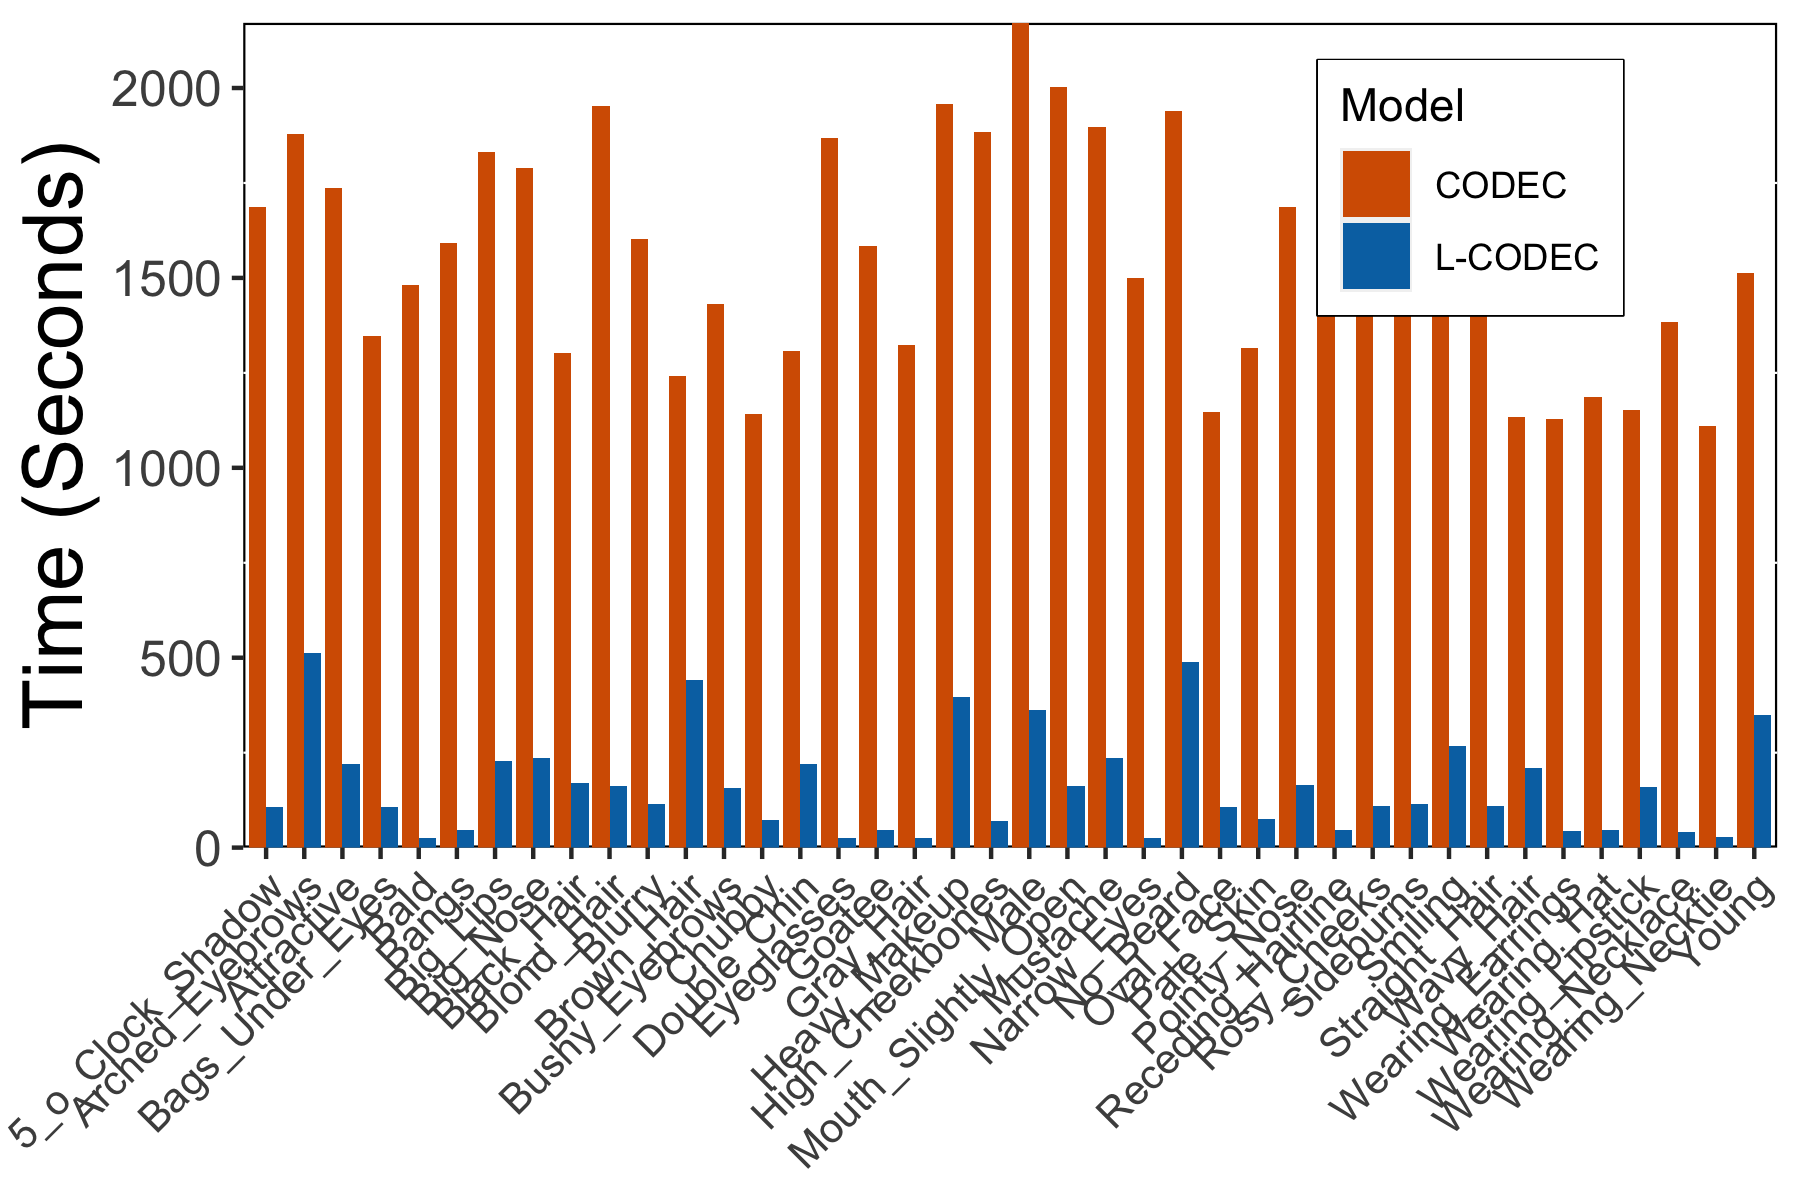
\includegraphics[width=\columnwidth]{5_unlearn/figs/Speed_Hist.png}
    \caption{\label{fig:full_speed_hist} L-CODEC vs CODEC run time comparison for identifying sufficient subsets for each CelebA attribute separately (pairs of columns, details in supplement).}
\end{figure}

\subsection{MNIST Toy Results}
Training for MNIST Logistic Regressor models was run using SGD with a learning rate of 0.1, batch size of 256, and weight decay of $0.01$ for 50 epochs. 1000 perturbations were used for distribution approximation. Privacy parameters were set to $\epsilon=0.1, \delta=0.01$.
Figures and numbers in the main thesis were averaged over 10 replications, for a random choice of 1000 samples to scrub.

\subsection{Retraining Comparisons}
\subsubsection{MNIST: Affects of $l_2$ Regularization and Weight Decay}
Repeating the retraining comparison in the main thesis with a larger regularization, we see that the effects of removal are significantly diminished and the model can support a larger number of removals before large performance drops.
\begin{figure}
    \centering
    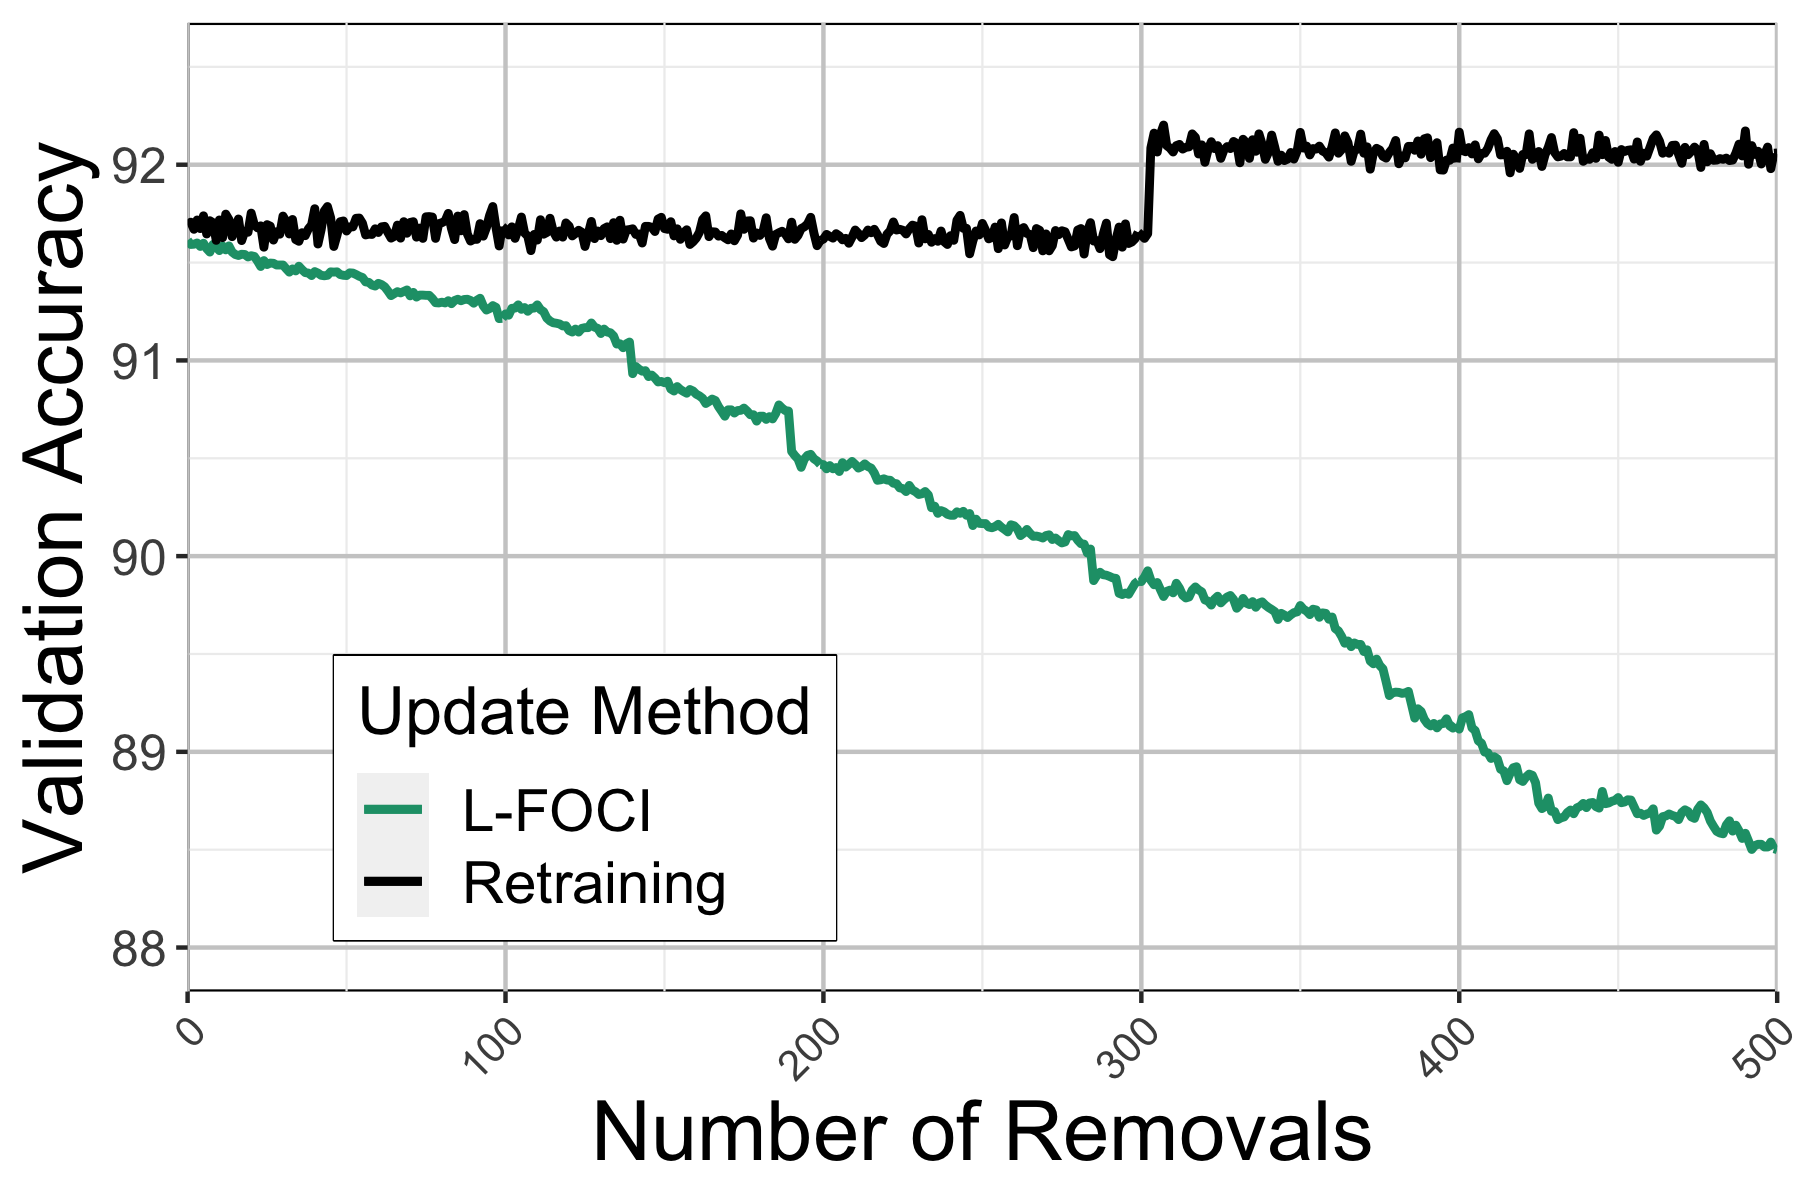
\includegraphics[width=0.24\columnwidth]{5_unlearn/figs/retrain/Retrain_Validation_Accs_0.01.png}
    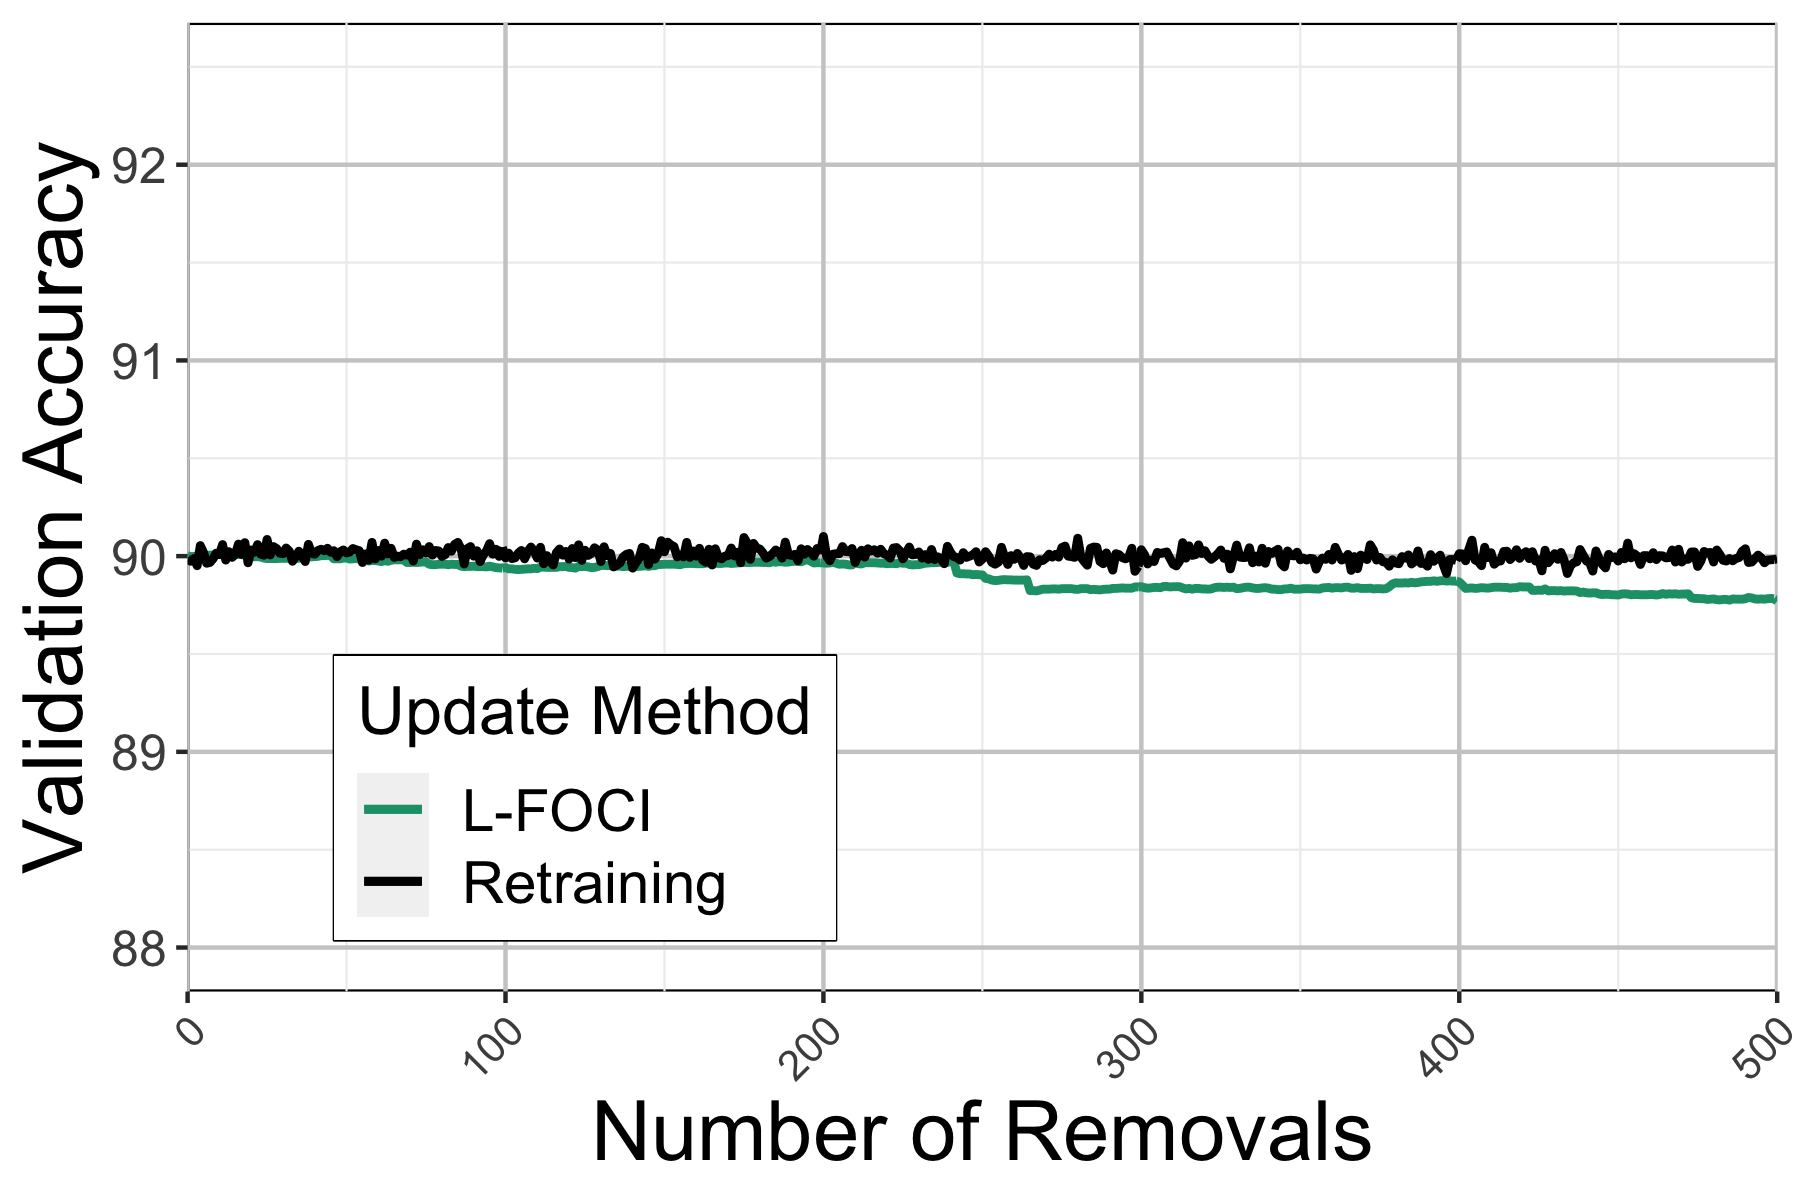
\includegraphics[width=0.24\columnwidth]{5_unlearn/figs/retrain/Retrain_Validation_Accs_0.1.png}
    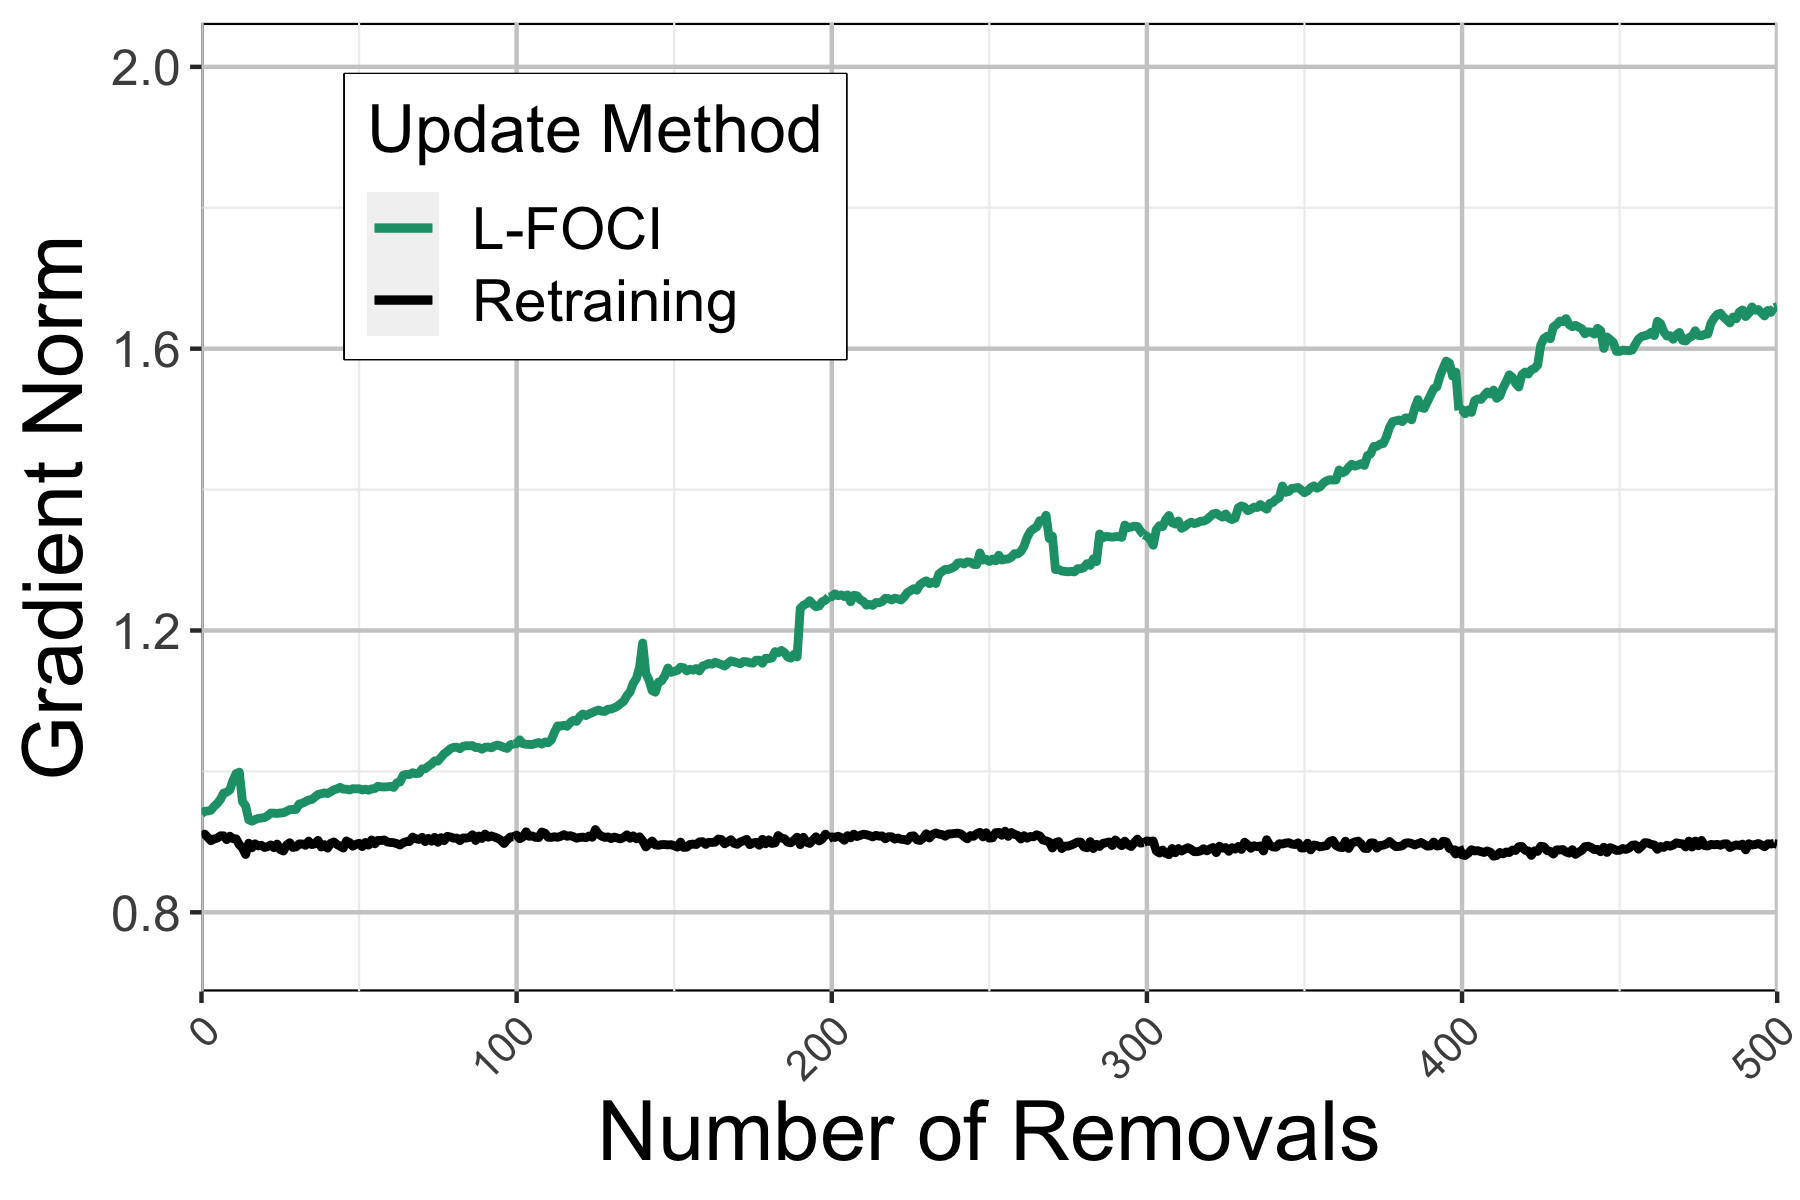
\includegraphics[width=0.24\columnwidth]{5_unlearn/figs/retrain/Retrain_Gradient_Norms_0.01.png}
    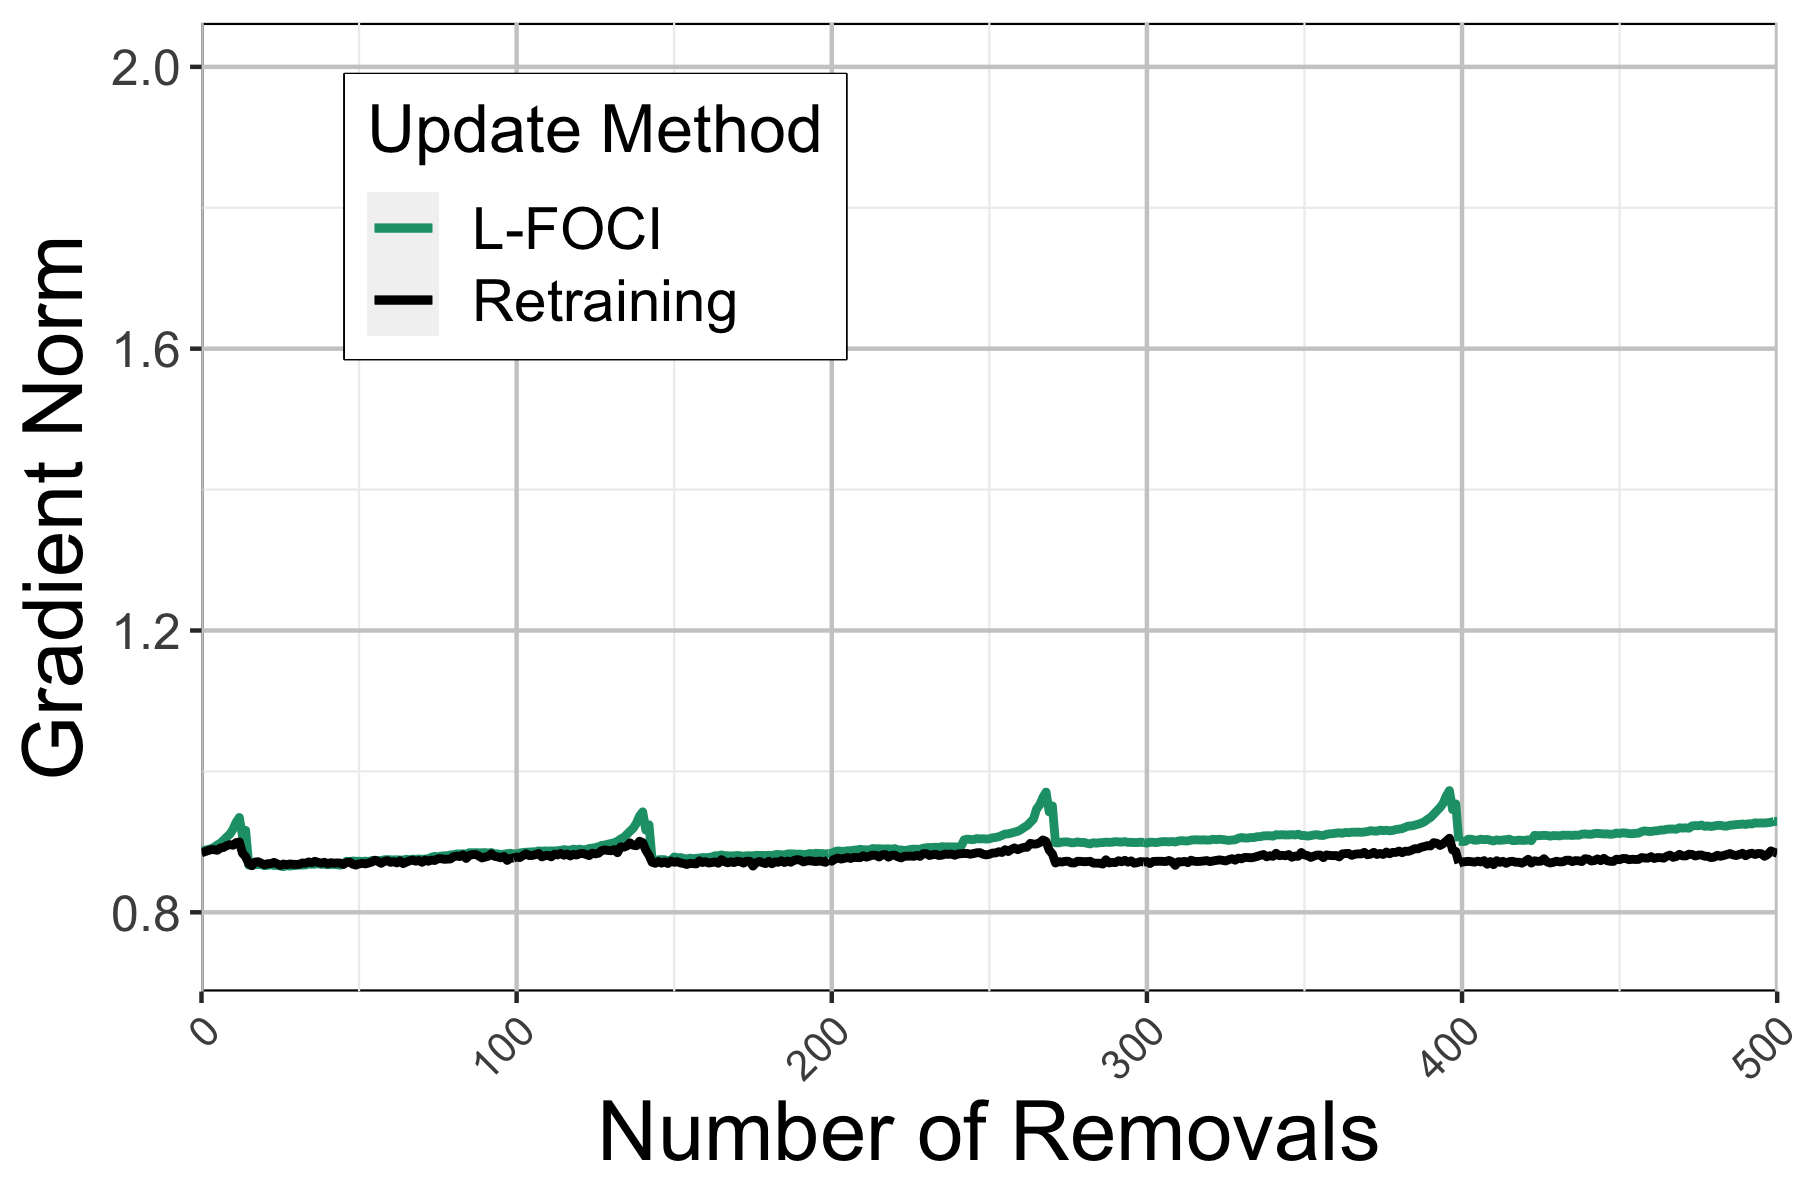
\includegraphics[width=0.24\columnwidth]{5_unlearn/figs/retrain/Retrain_Gradient_Norms_0.1.png}
    \caption[MNIST Retraining results]{MNIST Retraining results, comparing the effect of weight decay on unlearning via our LFOCI unlearning scheme and retraining.}
    \label{fig:mnistretrainweightdecay}
\end{figure}

\subsubsection{CIFAR Retraining Comparisons: A Note on Batch Normalization}
An important requirement for our retraining experiment is that our residual training set used for both scrubbing validation and retraining is able to take on any size, including 1 and any size for which the modulus over the batch size equals 1. This causes particular problems when models include batch normalization layers: general practice in training deep neural networks includes the choice of dropping the last batch, so as to avoid issues of unbalanced batch sizes. For our setting we \textit{cannot} drop these batches, because we explicitly want to measure and compute on networks trained with and without specific samples. While we can ``skip" removals during our experimentation, this can still lead to odd behavior, see Figure~\ref{fig:cifarretrain}. The spikes are exactly congruent with points in the removal process corresponding to a final batch size of 1 for retraining. In general, care must be taken when attempting to unlearn from batchnorm models, and further work may be necessary to adequately address it, both in theory and practice.
\begin{figure}
    \centering
    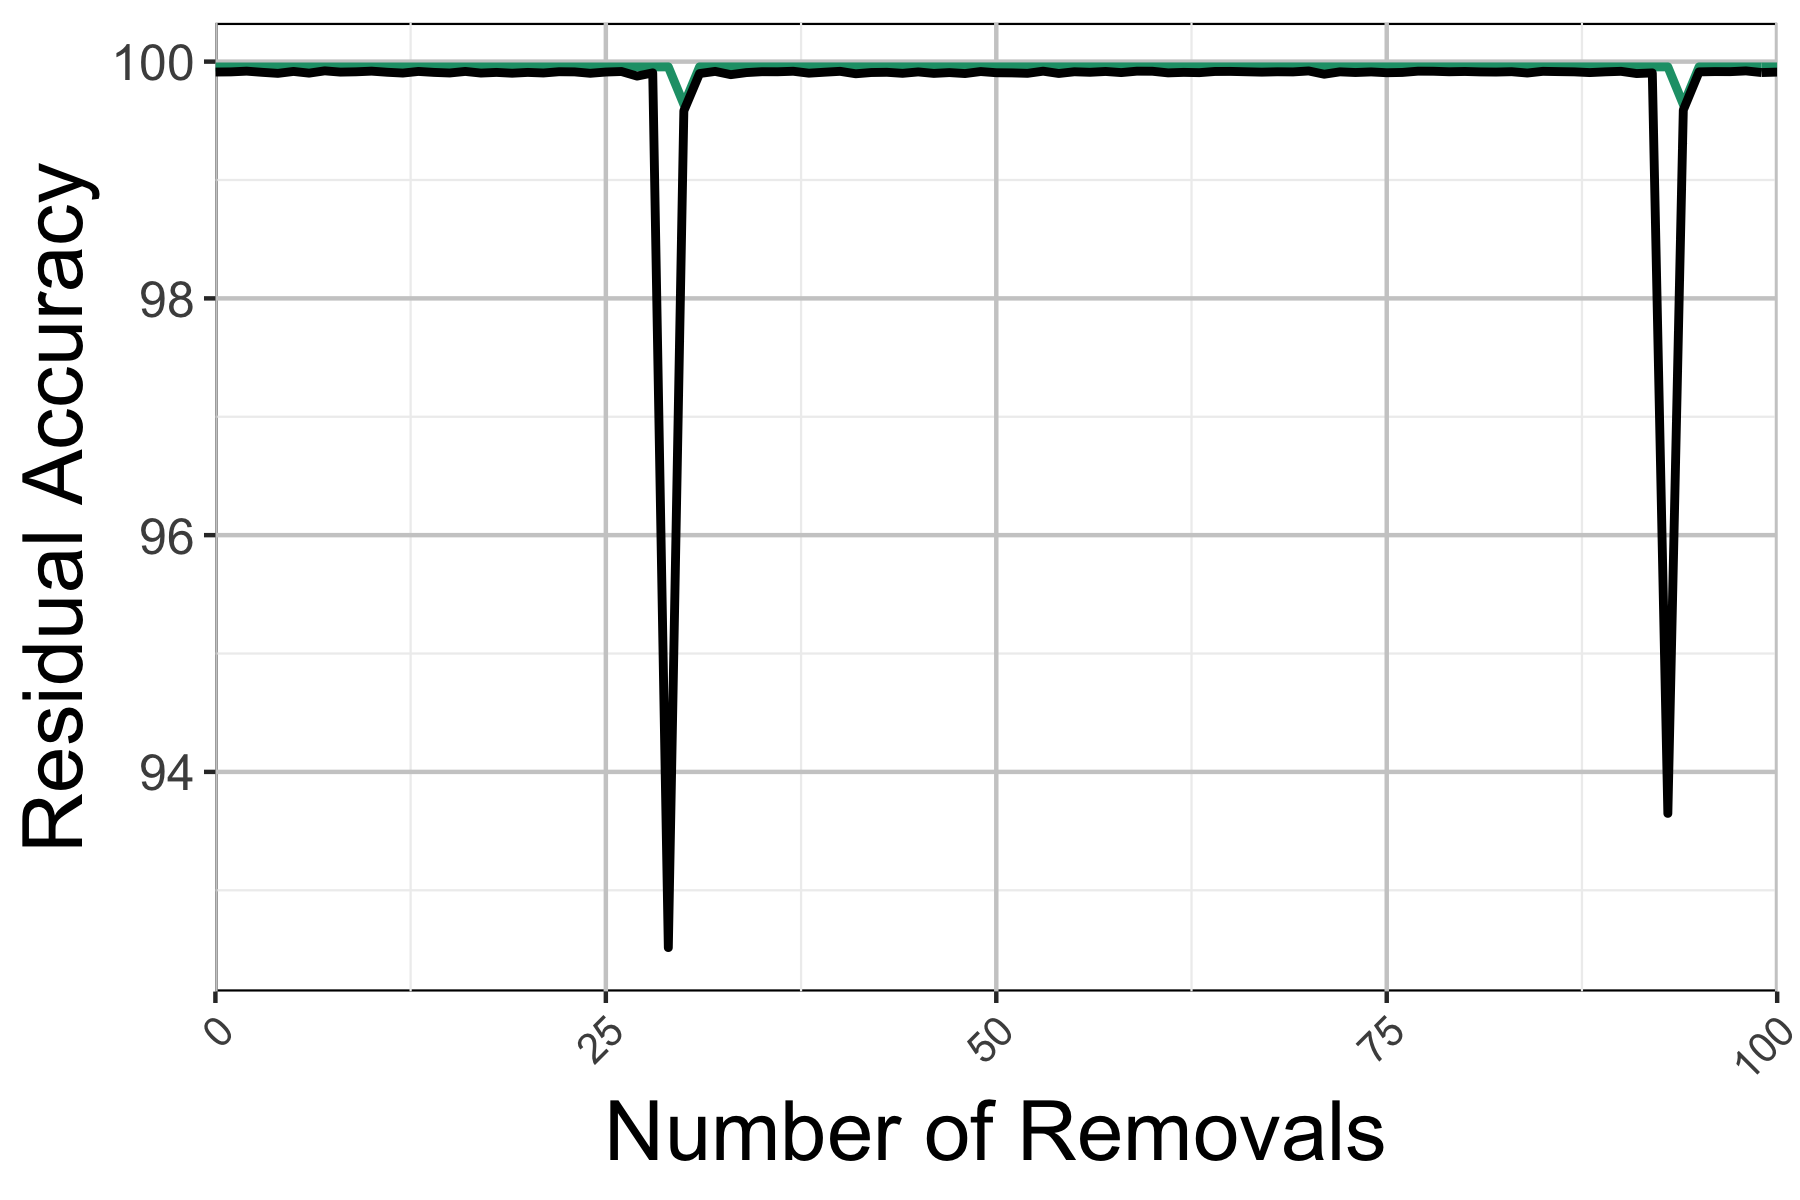
\includegraphics[width=0.495\columnwidth]{5_unlearn/figs/retrain/CIFAR_Retrain_Residual_Accs.png}
    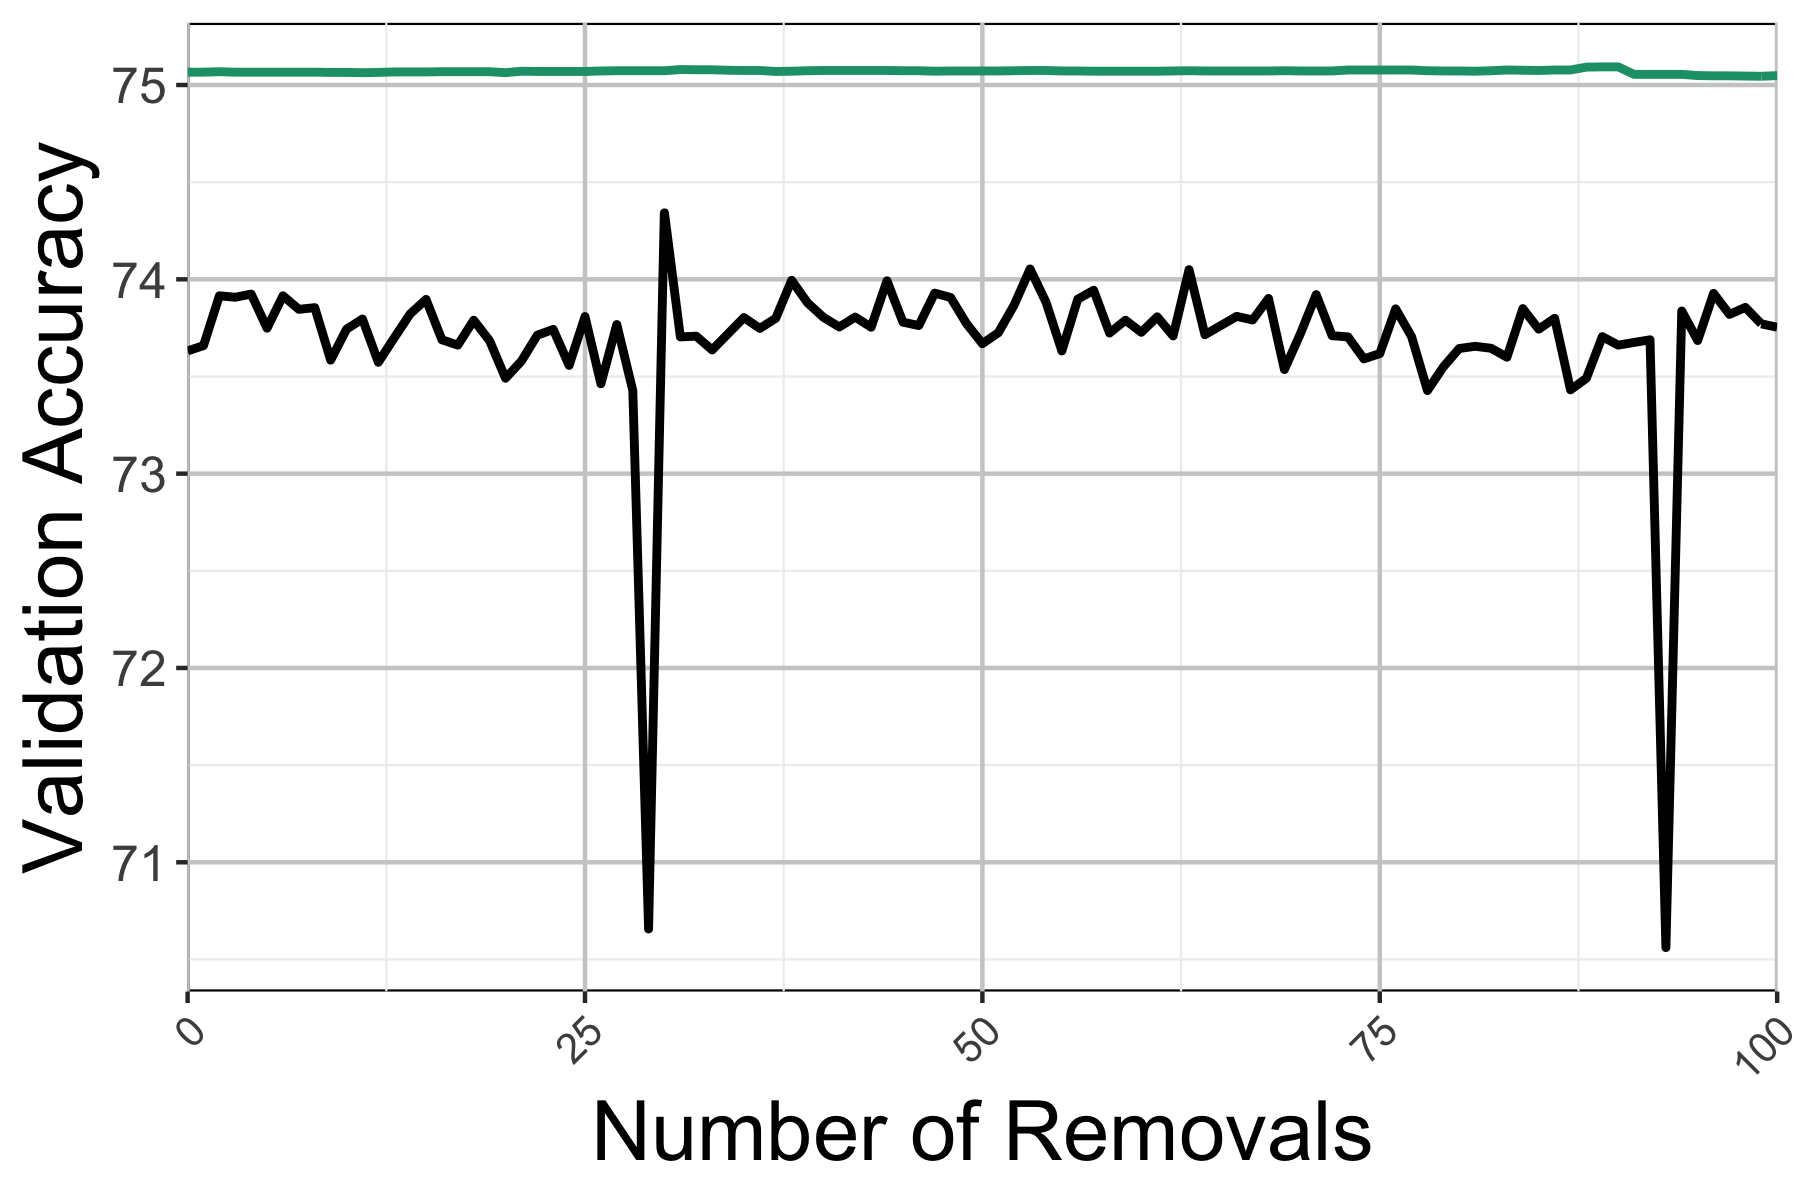
\includegraphics[width=0.495\columnwidth]{5_unlearn/figs/retrain/CIFAR_Retrain_Validation_Accs.png}
    \caption[CIFAR retraining results]{Retraining Results on CIFAR. Dips occur at removal counts where the modulus equals 1.}
    \label{fig:cifarretrain}
\end{figure}

\subsection{CIFAR-10 Model Comparisons}
Models were trained using Torch Hub, with a batch size of 64, learning rate of 0.1 for all models except VGG-11/bn, for which 0.01 was used. Data augmentation was NOT used, and weight decay was set to $0.01$.
1000 perturbations were used for distribution approximation. Privacy parameters were set to $\epsilon=0.1, \delta=0.01$.
Figures and numbers in the main thesis were averaged over 2 replications, for a random choice of 1000 samples to scrub.

\subsection{LEDGAR DistillBERT Details}
For the NLP experiments, we used a pretrained model from HuggingFace as a starting point. Specifically, we used the transformer model ``distilbert-base-uncased", \url{https://huggingface.co/distilbert-base-uncased} which is a distilled version of the BERT base model, smaller and faster than BERT. It was pretrained on the same corpus in a self-supervised fashion, using the BERT base model as a teacher. DistilBERT \cite{sanh2019distilbert} was pretrained on the raw texts only, without any human labels. The three losses used for the pre-training are that of distillation loss, masked language modelling and cosine embedding loss. This pre-trained model was then fine-tuned for the downstream task of provision classification using the LEDGAR dataset introduced in \citep{tuggener2020ledgar}. We used the prototypical dataset which had 13 most common labels based on frequency. The model was fine-tuned for 4 epochs, updating all of it's parameters without any freezing based on binary cross entropy loss with class weighting. The labels were converted to one-hot vectors and hence binary cross entropy loss was used. Learning rate used was $5e^{-5}$ and weight decay of $0.01$. No weight decay was applied for bias and normalization layer parameters. We used batch size of 256 and restricted the maximum length of tokens to $128$ per data point. Further gradients were clipped based on the infinity norm to a value of $1.0$. We used AdamW optimizer with an epsilon value of $1e^{-8}$; and the learning rate scheduler used was WarmupLinearSchedule both from PyTorch\_Transformers. 

For unlearning experiments on this model, we remove provisions pertaining to a specific class. We removed samples from two classes namely ``Governing Laws" and ``Terminations" which had the highest and lowest support respectively. We were able to removed a varying number of samples from these classes based on the selection of the privacy parameter of $\epsilon$ for scrubbing. The results are tabulated in the main part of the thesis.

\subsection{VGG-Face Identification Scrubbing}
For this setting, the trained model was downloaded from \url{https://www.robots.ox.ac.uk/~vgg/data/vgg_face/} and converted to PyTorch via \url{https://github.com/prlz77/vgg-face.pytorch}. A partial version of the dataset was constructed using the list of image URLs, consisting of 100 images for each identity within the set. The images were processed as described in the original paper~\citep{Parkhi15}.

Fine tuning was done for 4 epochs to estimate the Hessian for the sample downloaded using SGD with a learning rate of $0.0001$ and a weight decay/$l_2$ regularization of $0.01$, with a batch size of 16.

For unlearning, 100 images for a specific identity were randomly ordered and removed with $\epsilon=0.0001, \delta=0.01$. 100 perturbations were used to estimate the activation and loss distributions for L-FOCI.

\subsection{Person Re-identification}
We discuss in more detail the experimental details of unlearning deep neural networks for the person re-identification task in this section. We consider four different datasets namely, Market1501 \citep{zheng2015scalable}, MSMT17 \citep{wei2018person}, PRID \citep{hirzer11} and  QMUL GRID \citep{loy2009multi}. We unlearn from different deep neural networks including ResNet50, a variant of ResNet50 with a fully connected layer (called Resnet50\_fc512), Multi-Level Factorisation Net (MLFN) and MobilNet\_V2. In all cases the models were first trained to reasonable accuracy as per benchmarks before proceeding with unlearning a randomly selected individual's identity from the corresponding dataset. To perform experiments pertaining to person re-identification we make use of the popular framework torchreid \citep{zhou2019omni}. We had to make changes to the original code in order to make our procedure function correctly in this framework. We include this modified source within the code presented in the supplement. We use Adam as the optimizer, a step scheduler and learning rate of $0.0003$ across all person re-identification datasets and models used. We use softmax loss and weights were initialized using a model pre-trained on ImageNet in all cases. Images were resized to $256 \times 128$ before being used as input to any of the models. The number of training epochs was chosen accordingly to allow the training to have converged. Results from multiple runs involving different models, datasets and the privacy parameter $(\epsilon)$ are conclusive. With lower value of $\epsilon$, e.g. $0.0005$, the number of samples that could be unlearned for a particular class while maintaining model performance was lower than what could be unlearned for a higher value of the privacy parameter $\epsilon$, e.g. $0.1$. For the smaller datasets, i.e. PRID and QMUL GRID, which have approximately 2 samples per class, the unlearning procedure lead to more drastic changes as expected and it could be observed that our selection procedure selected many more layers to update than what it did for the larger datasets. Activation maps from some experiments are presented in Figure~\ref{fig:reid_sup}.

\begin{figure*}
    \centering
    
    \begin{subfigure}[b]{0.98\textwidth}
        \centering
        \includegraphics[width=0.45\columnwidth]{5_unlearn/figs/scrub/0006_mlfn_rem1.jpg}
        \hspace{15pt}
        \includegraphics[width=0.45\columnwidth]{5_unlearn/figs/scrub/0001_mlfn_ret1.jpg}
    \end{subfigure}
    
    \vspace{5 pt}
    
    \begin{subfigure}[b]{0.98\textwidth}
        \centering
        \includegraphics[width=0.45\columnwidth]{5_unlearn/figs/scrub/0006_mlfn_rem2.jpg}
        \hspace{15pt}
        \includegraphics[width=0.45\columnwidth]{5_unlearn/figs/scrub/0029_mlfn_ret2.jpg}
    \end{subfigure}
    
    \vspace{5 pt}
    
    \begin{subfigure}[b]{0.98\textwidth}
        \centering
        \includegraphics[width=0.45\columnwidth]{5_unlearn/figs/scrub/0006_mob_rem1.jpg}
        \hspace{15pt}
        \includegraphics[width=0.45\columnwidth]{5_unlearn/figs/scrub/0014_mob_ret1.jpg}
    \end{subfigure}
    
    \vspace{5 pt}
    
    \begin{subfigure}[b]{0.98\textwidth}
        \centering
    \subfloat[\centering Scrubbed class]{{\includegraphics[width=0.45\columnwidth]{5_unlearn/figs/scrub/0006_mob_rem2.jpg}}}%
    \hspace{15pt}
    \subfloat[\centering Unscrubbed class]{{ \includegraphics[width=0.45\columnwidth]{5_unlearn/figs/scrub/0026_mob_ret2.jpg}}}%
    
        % \includegraphics[width=0.4\columnwidth]{figs/scrub/0006_mob_rem2.jpg}
        % \caption{One part}
        
        % \includegraphics[width=0.49\columnwidth]{figs/scrub/0026_mob_ret2.jpg}
        % \caption{Two part}
    \end{subfigure}
    
    % \hspace{1pt}
    
    % \begin{subfigure}[b]{1.0\textwidth}
    %     % \includegraphics[width=0.49\columnwidth]{figs/scrub/0006_mob_rem2.jpg}
    %     % \caption{One part}
        
    %     \includegraphics[width=0.4\columnwidth]{figs/scrub/0026_mob_ret2.jpg}
    %     \caption{Two part}
    % \end{subfigure}
    
    %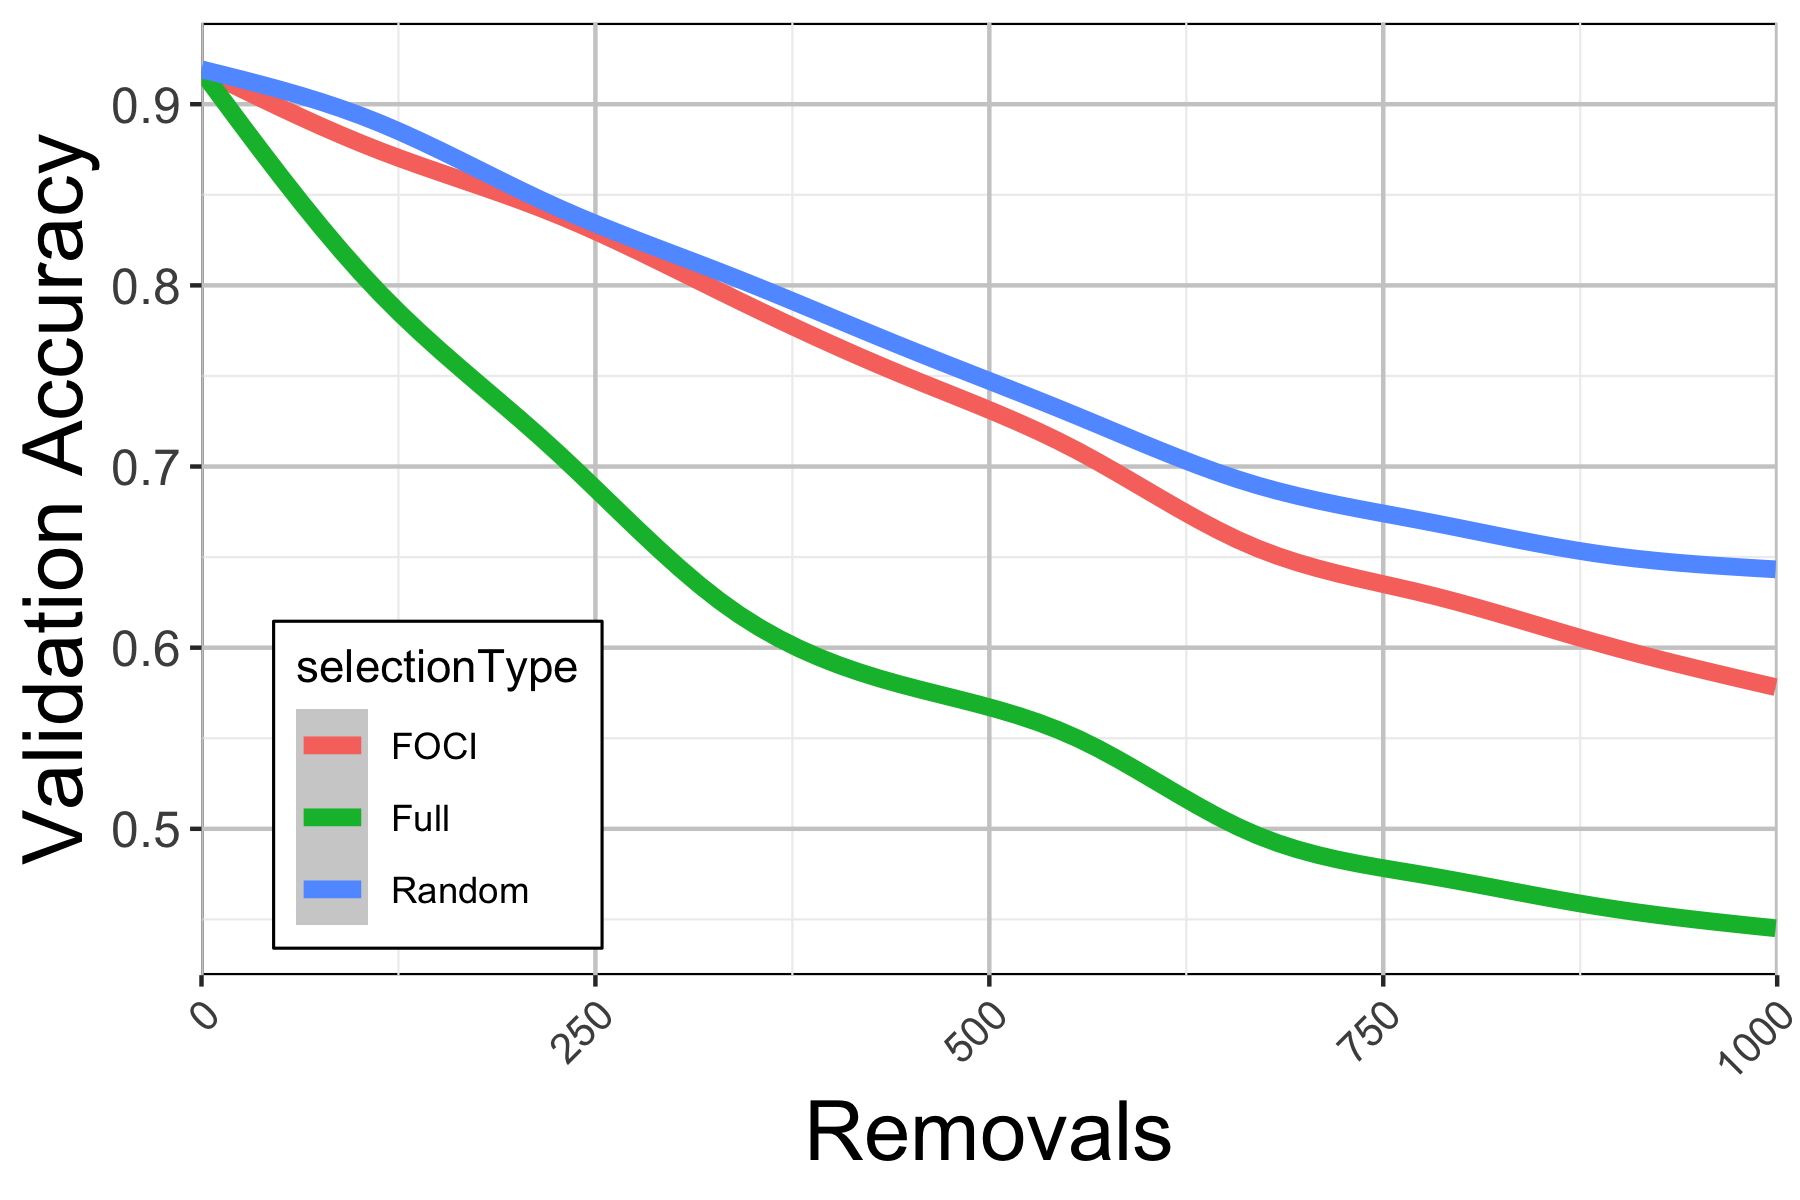
\includegraphics[width=0.3\textwidth]{figs/scrub/MNIST_Valid_Acc.png}
    
    % \vspace{-10pt}
    \caption[Re-ID Activation Maps]{\label{fig:reid_sup}Activation maps from different models (top two rows MLFN, bottom two MobileNet\_V2; both trained on Market\_1501) scrubbed for the person on the left. For each triplet, from (L to R) are the original image, the activation map and its image overlay. Activations change significantly for the scrubbed sample (compare column 2 to 3) whereas remain stable for the non-scrubbed sample (compare column 5 to 6).}
\end{figure*}




% \begin{figure}[!tb]
%     \centering
%     %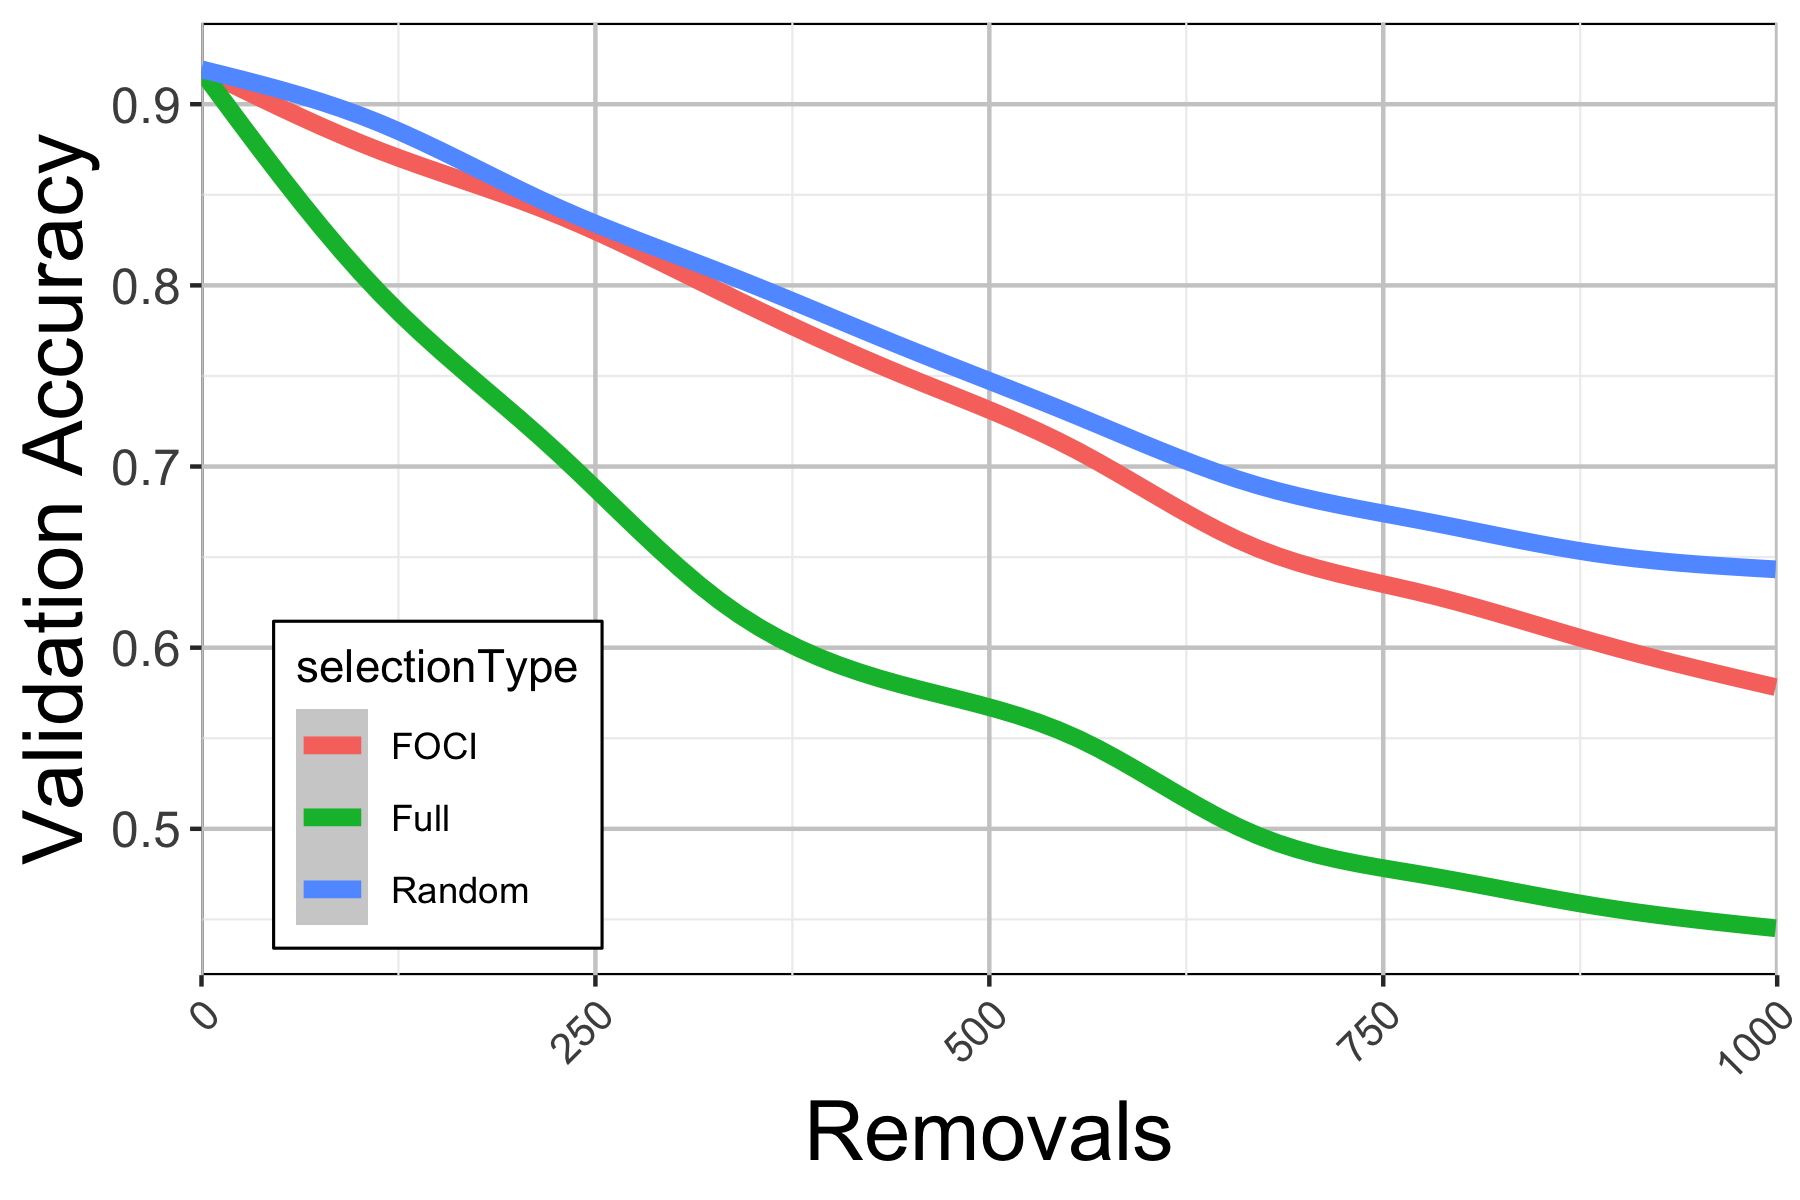
\includegraphics[width=0.3\textwidth]{figs/scrub/MNIST_Valid_Acc.png}
%     \includegraphics[width=0.49\columnwidth]{figs/scrub/0006_mlfn_rem1.jpg}
%      \includegraphics[width=0.49\columnwidth]{figs/scrub/0001_mlfn_ret1.jpg}
%      \vspace{-10pt}
%     \caption{\label{fig:reid}Activation maps from a MLFN model scrubbed for the person on the left (right set is not scrubbed). For each triplet, from (L to R) are the original image, the activation map and its image overlay. Note the effect of scrubbing: activations change significantly for the scrubbed sample (compare column 2 to 3) whereas remain stable for the non-scrubbed sample (compare column 5 to 6).}
% \end{figure}

% \begin{figure}[!tb]
%     \centering
%     %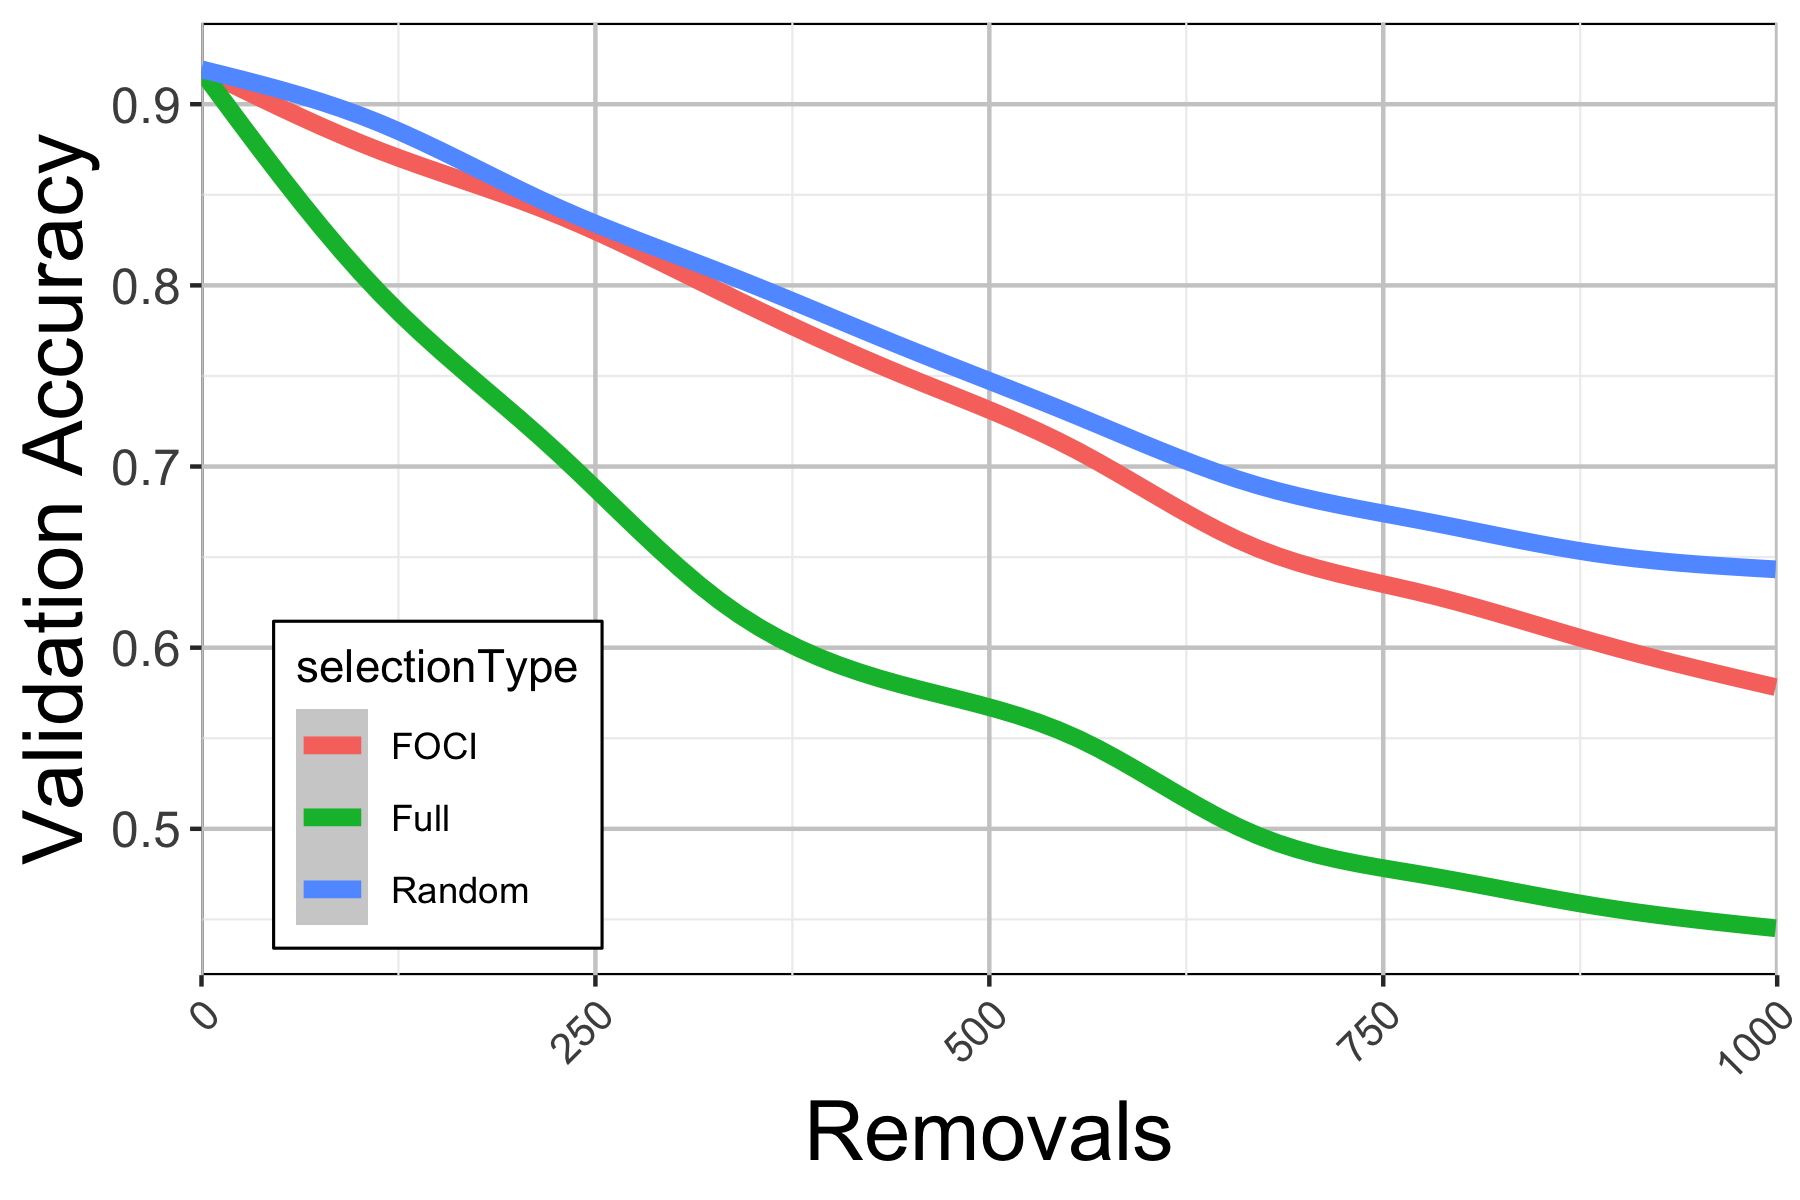
\includegraphics[width=0.3\textwidth]{figs/scrub/MNIST_Valid_Acc.png}
%     \includegraphics[width=0.49\columnwidth]{figs/scrub/0006_mlfn_rem2.jpg}
%      \includegraphics[width=0.49\columnwidth]{figs/scrub/0029_mlfn_ret2.jpg}
%      \vspace{-10pt}
%     \caption{\label{fig:reid}Activation maps from MLFN model scrubbed for the person on the left (right set is not scrubbed). For each triplet, from (L to R) are the original image, the activation map and its image overlay. Note the effect of scrubbing: activations change significantly for the scrubbed sample (compare column 2 to 3) whereas remain stable for the non-scrubbed sample (compare column 5 to 6).}
% \end{figure}

% \begin{figure}[!tb]
%     \centering
%     %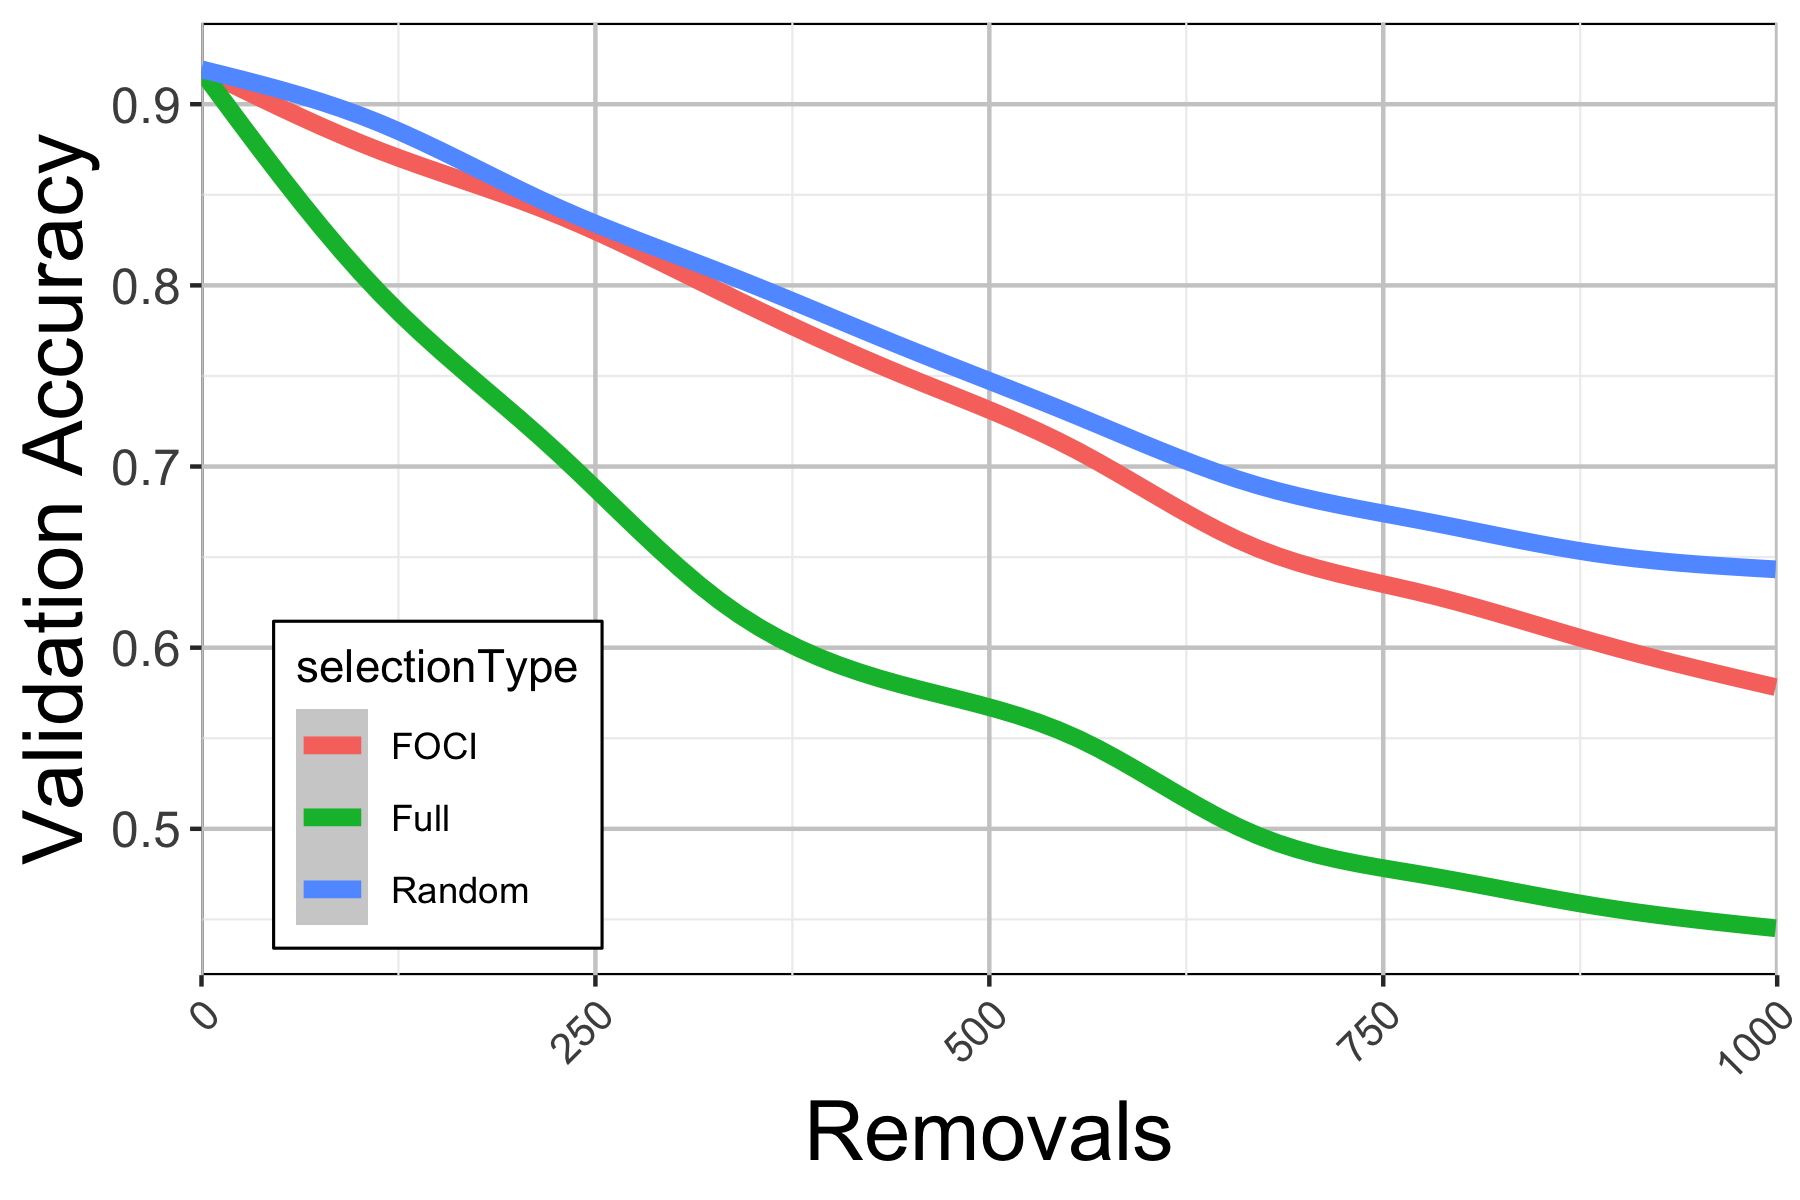
\includegraphics[width=0.3\textwidth]{figs/scrub/MNIST_Valid_Acc.png}
%     \includegraphics[width=0.49\columnwidth]{figs/scrub/0006_mob_rem1.jpg}
%      \includegraphics[width=0.49\columnwidth]{figs/scrub/0014_mob_ret1.jpg}
%      \vspace{-10pt}
%     \caption{\label{fig:reid}Activation maps from MobileNet\_V2 model scrubbed for the person on the left (right set is not scrubbed). For each triplet, from (L to R) are the original image, the activation map and its image overlay. Note the effect of scrubbing: activations change significantly for the scrubbed sample (compare column 2 to 3) whereas remain stable for the non-scrubbed sample (compare column 5 to 6).}
% \end{figure}

% \begin{figure}[!tb]
%     \centering
%     %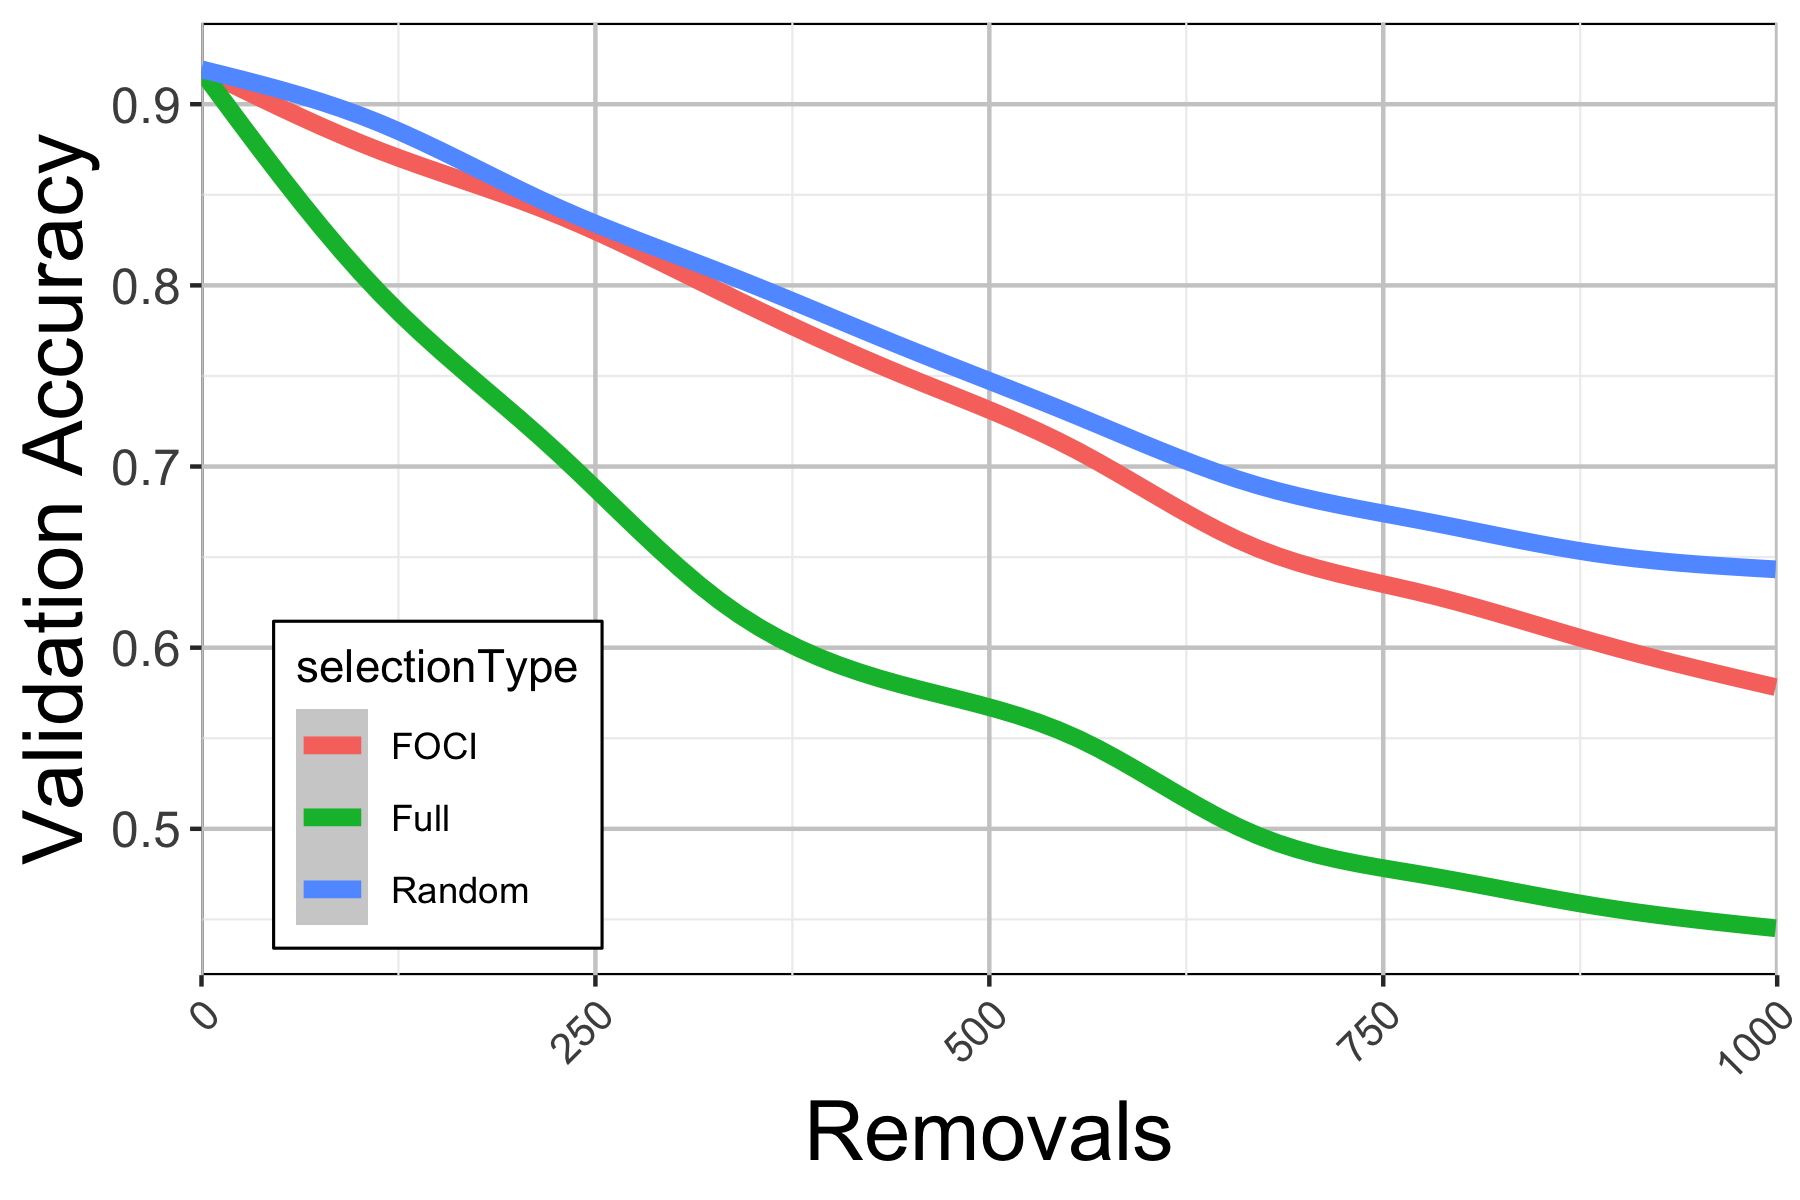
\includegraphics[width=0.3\textwidth]{figs/scrub/MNIST_Valid_Acc.png}
%     \includegraphics[width=0.49\columnwidth]{figs/scrub/0006_mob_rem2.jpg}
%      \includegraphics[width=0.49\columnwidth]{figs/scrub/0026_mob_ret2.jpg}
%      \vspace{-10pt}
%     \caption{\label{fig:reid}Activation maps from MobileNet\_V2 model scrubbed for the person on the left (right set is not scrubbed). For each triplet, from (L to R) are the original image, the activation map and its image overlay. Note the effect of scrubbing: activations change significantly for the scrubbed sample (compare column 2 to 3) whereas remain stable for the non-scrubbed sample (compare column 5 to 6).}
% \end{figure}

% \subsection{Dataset Details}

% \subsection{Spurious Feature Regularization.}
% This Markov Blanket identification scheme can also be used to address spurious feature effects on traditional NN models.
% %In modern machine learning applications, strict classification or regression on outcomes of interest is no longer sufficient to deploy models in the real world. 
% %Particularly, a large number of existing machine learning problems such as overfitting to spurious features and class imbalance can drastically affect model performance on biased training data. 
% % Removing the effect of spurious features can be achieved in many ways, but it requires knowledge of which features should be considered.
% % Here, we look at applications in which there may be a large number of outside factors, or side information, that may be heavily dependent, or spurious, to the outcome variable. 
% %Using typical tools in the ML toolbox,
% % A natural method of attempting to incorporate side information would be to add appropriate loss terms to the global objective, where the loss terms may be pushing the learning algorithm towards \textit{regularized} models that are further away from the training set optimum, but closer to the solution of the true question.
% A straightforward approach would be to directly add a loss term for each potentially important feature over which we would like to regularize, 
% \begin{align}
% \cL(\theta) + \sum_{S\in \cS} R_S(\theta)
% \end{align}
% However, in the case where the set of outside factors $S$ is large, these regularizers can adversely effect training, to the point where for any reasonable regularization parameter settings no model is able to be found with high performance on the outcome of interest. Using L-FOCI, we can instead identify the set of minimal factors that, when conditioned, make the rest conditionally independent. Then it is only necessary to include regularizers over $S \in MB(Y)$.
% %Here, if we consider a graph over the external factors and our outcome of interest, it is immediately clear that if we wish to regularize the effect of all factors, it is sufficient to only regularize the effect of the Markov Blanket. 
% % \begin{align}
% % \cL(\theta) + \sum_{S\in MB(Y)} R_S(\theta)
% % \end{align}

% We evaluate under a simple attribute image classification setting using the CelebA dataset. We run our L-FOCI algorithm over the attributes as in our L-CODEC evaluation, and regularize using a Gradient Reversal Layer for a simple accuracy term over those attributes.
% We compare models with varying regularization over all attributes, randomly chosen attributes, and FOCI-selected attributes.
% Figure \ref{fig:spur} shows these results. Clearly selection with FOCI provides the best result, maintaining high global accuracy while also holding high accuracy on sets of samples with and without correlated attributes.


% \begin{figure*}[t]
%     \centering
%     %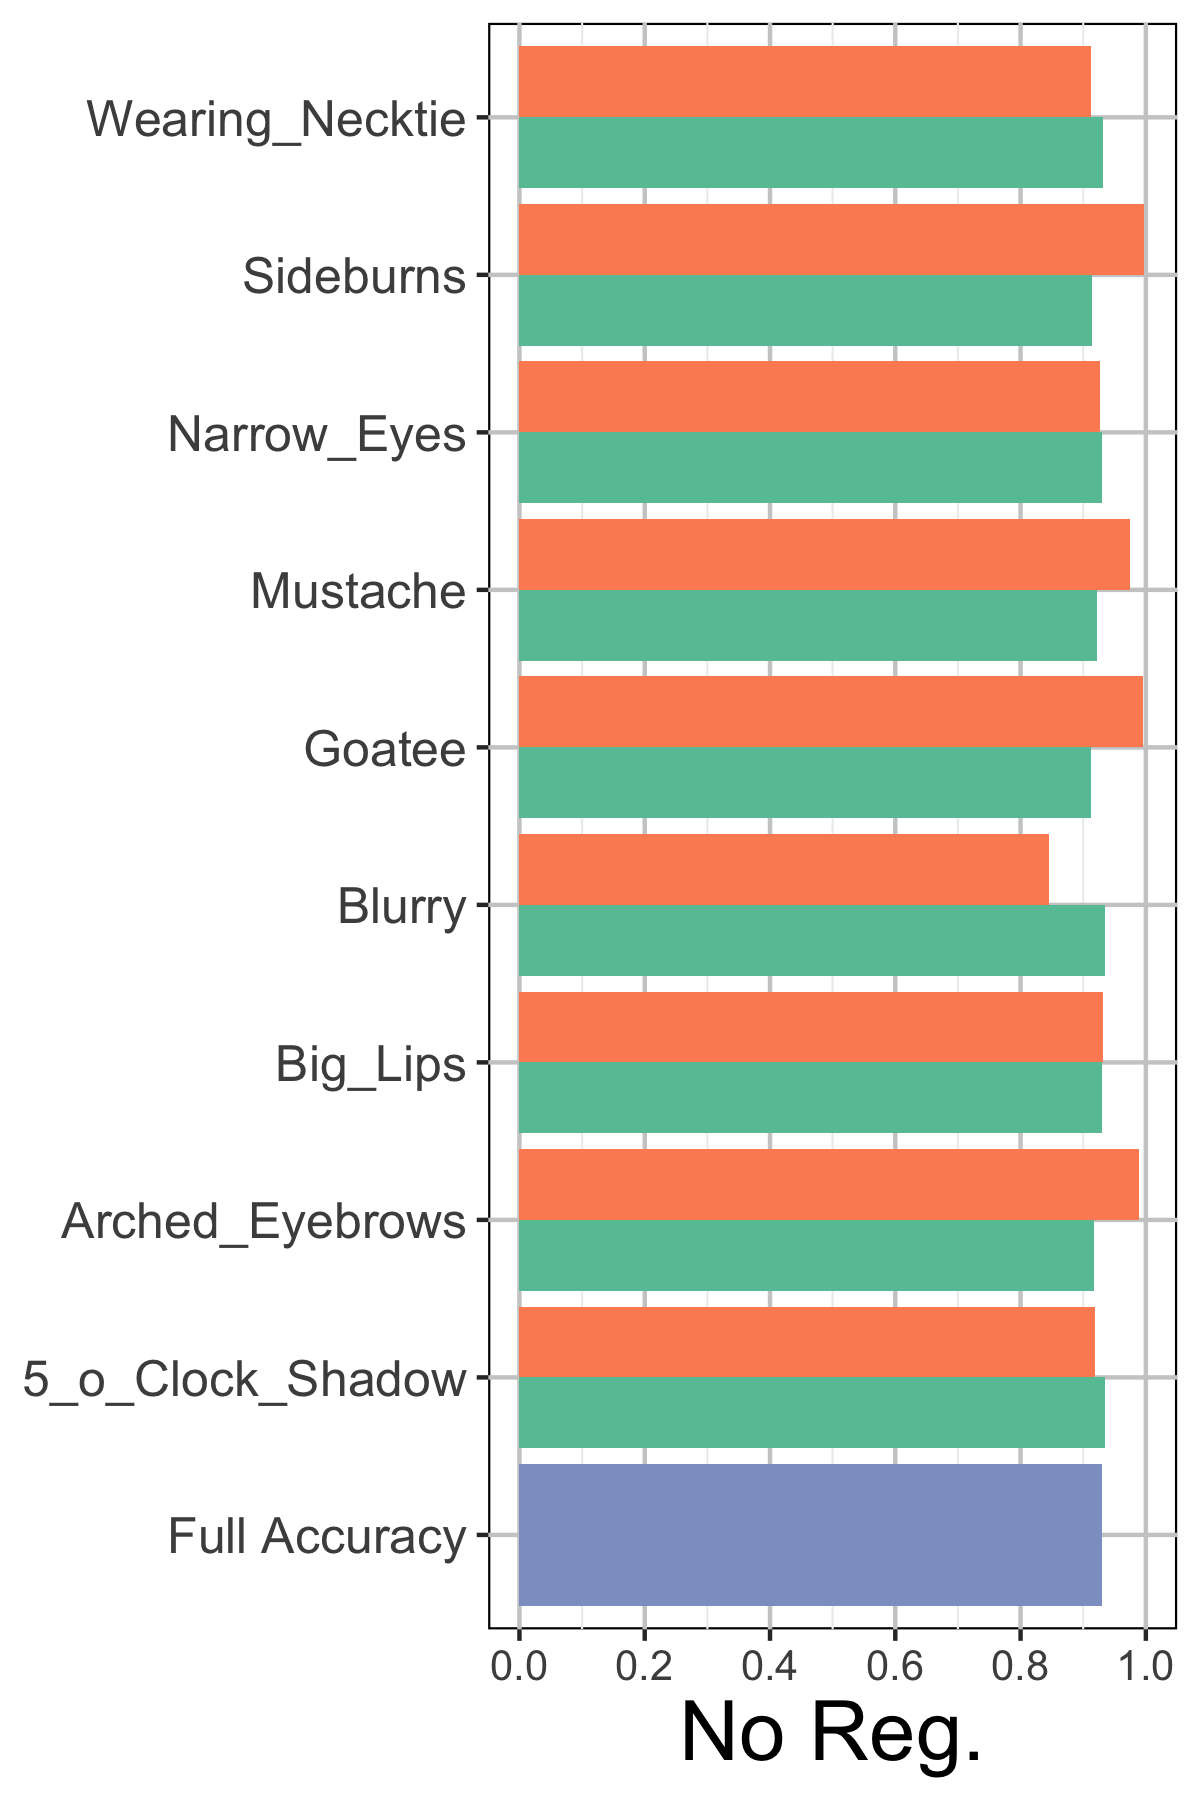
\includegraphics[width=0.24\textwidth]{figs/No_Beard_None.png}
%     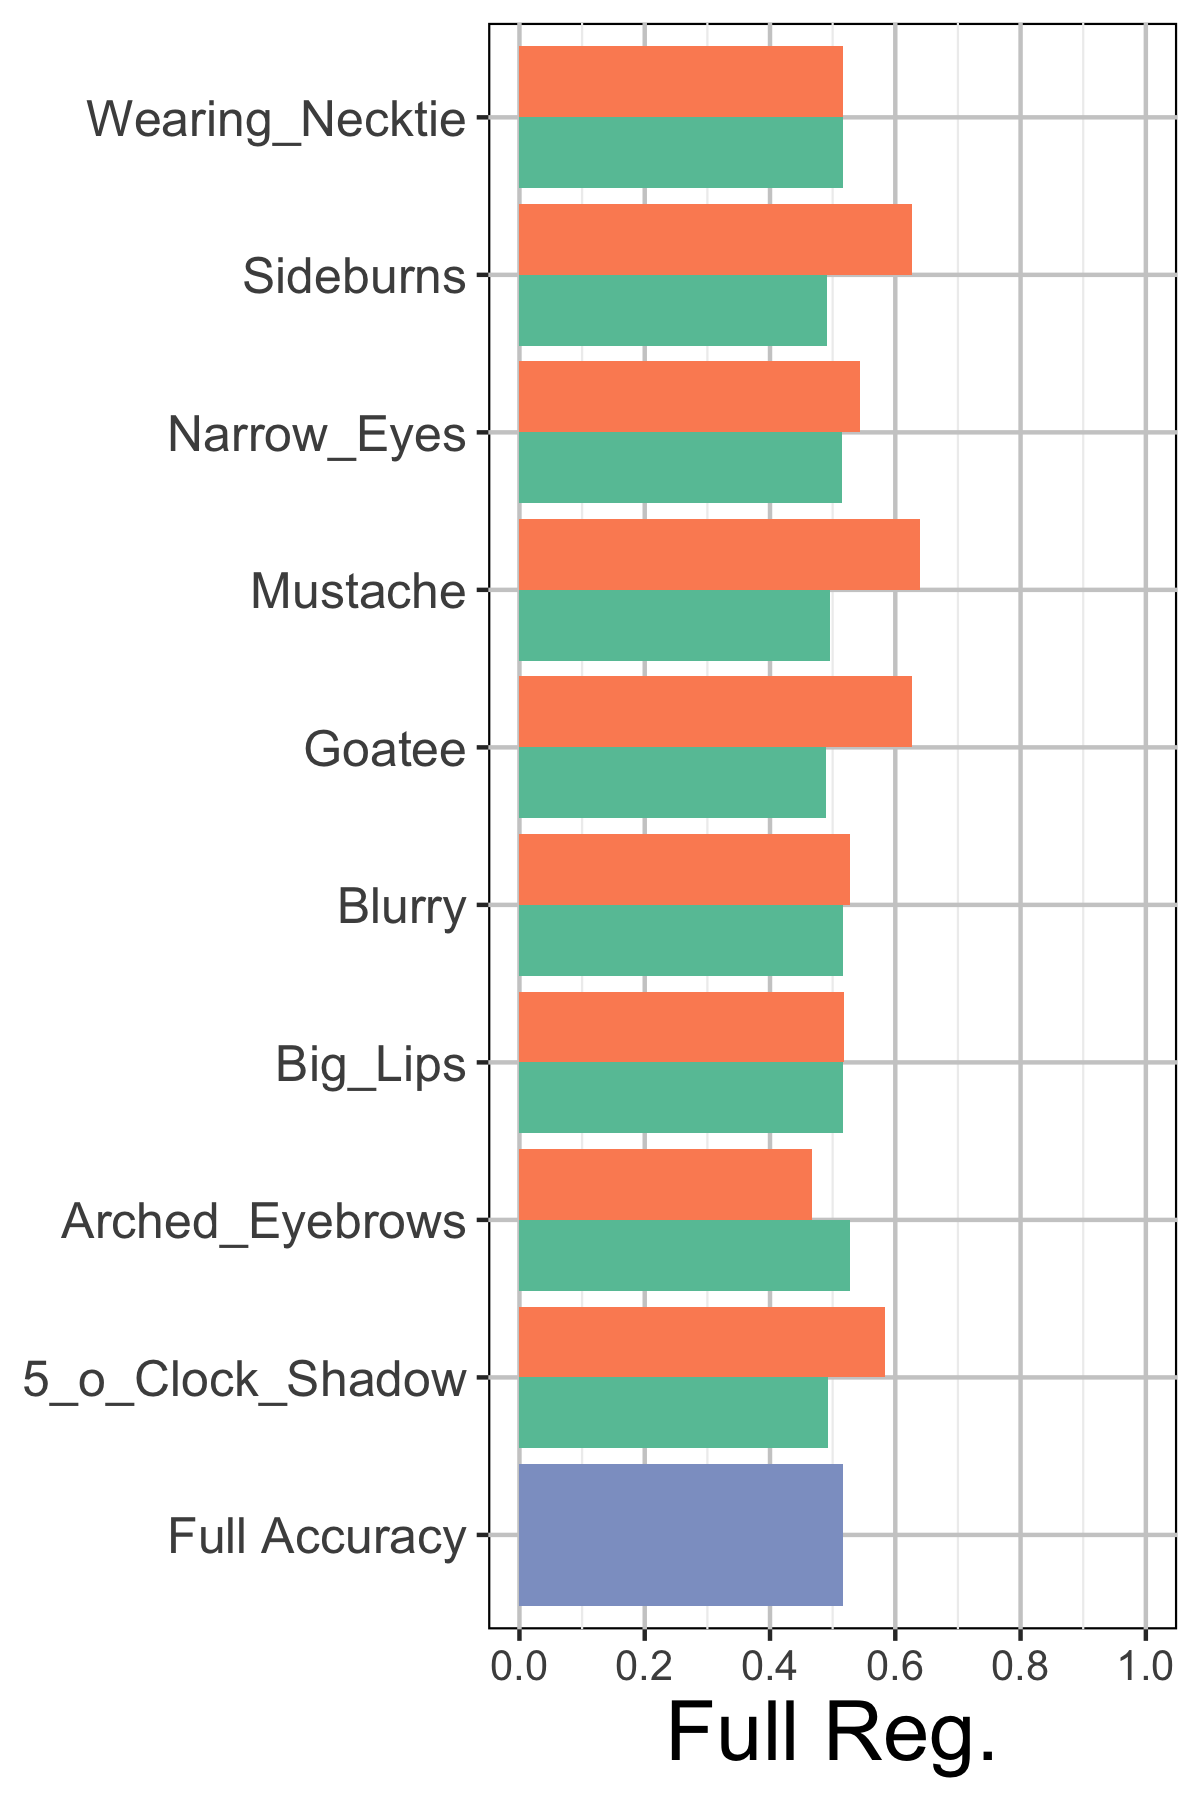
\includegraphics[width=0.3\textwidth]{figs/No_Beard_All.png}
%     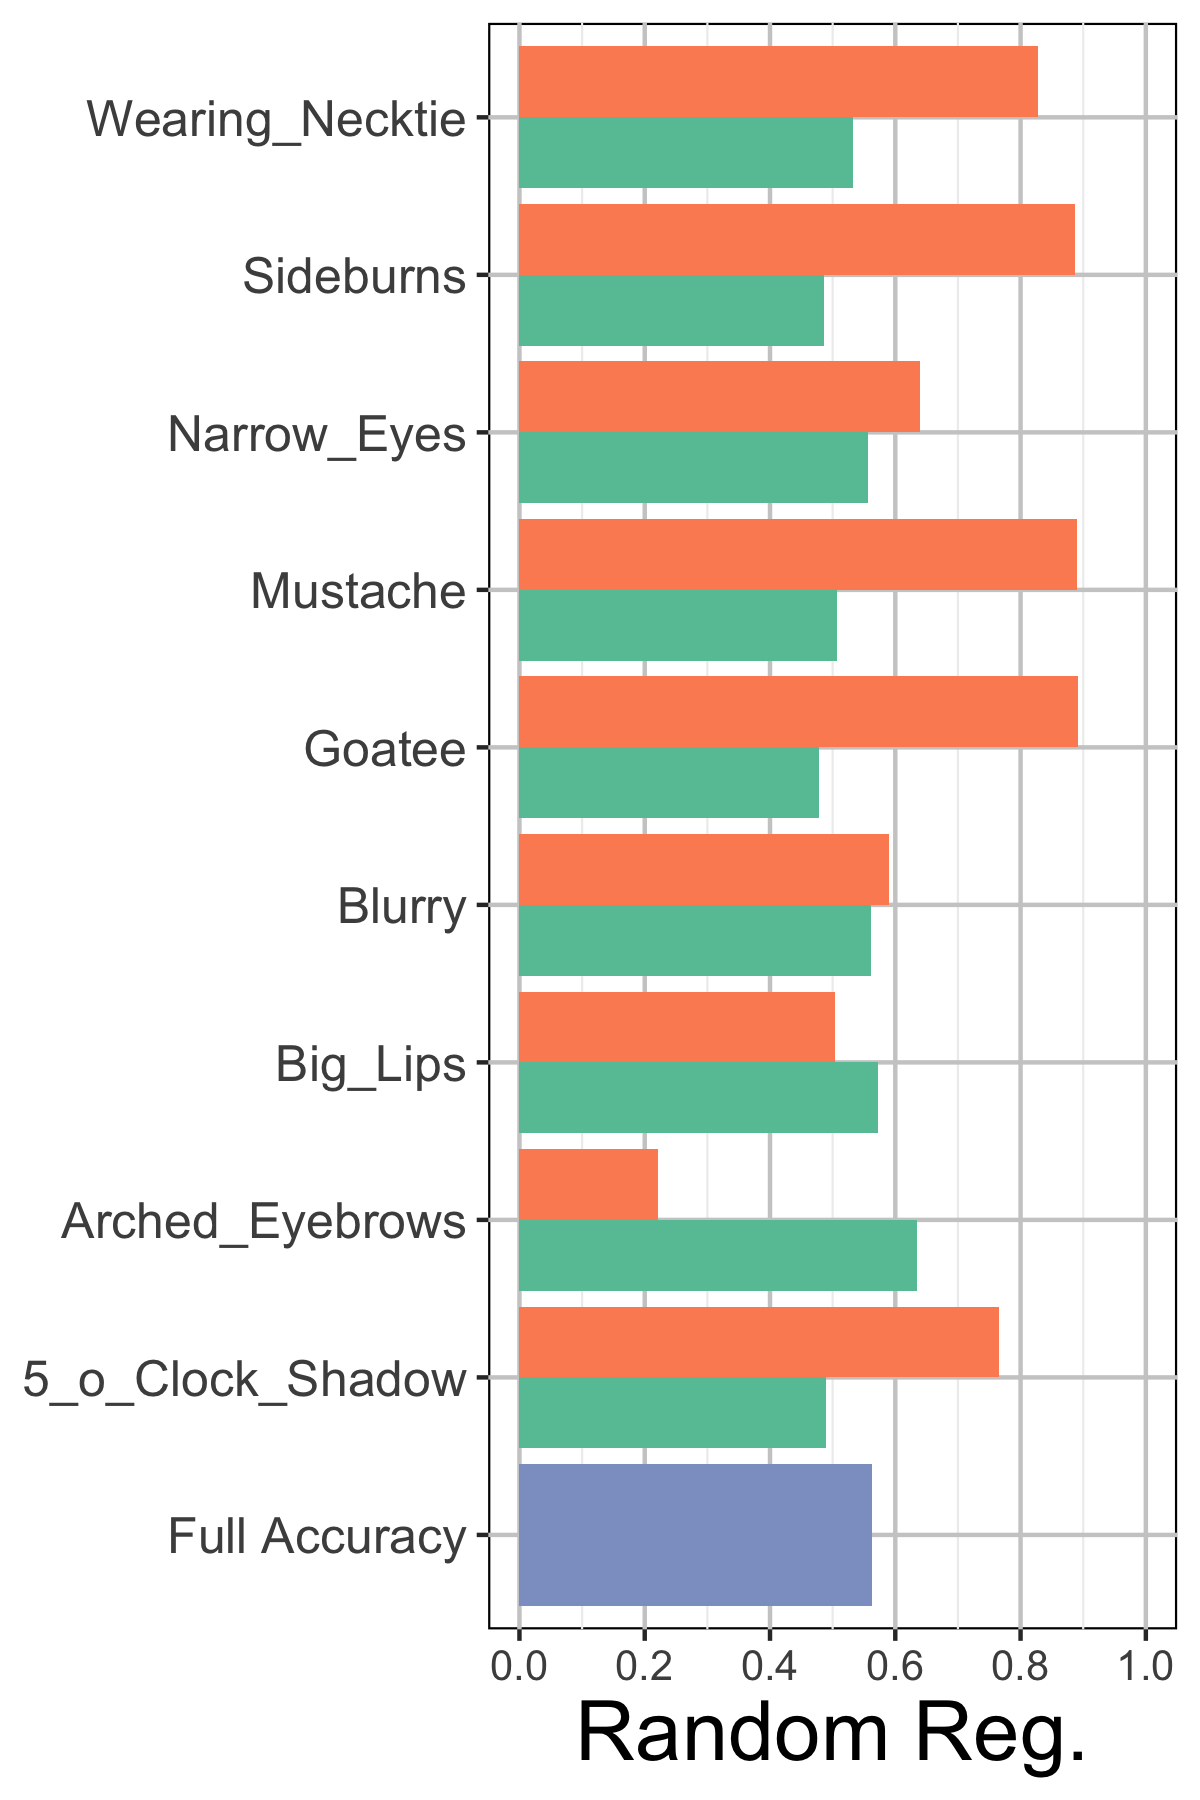
\includegraphics[width=0.3\textwidth]{figs/No_Beard_Random.png}
%     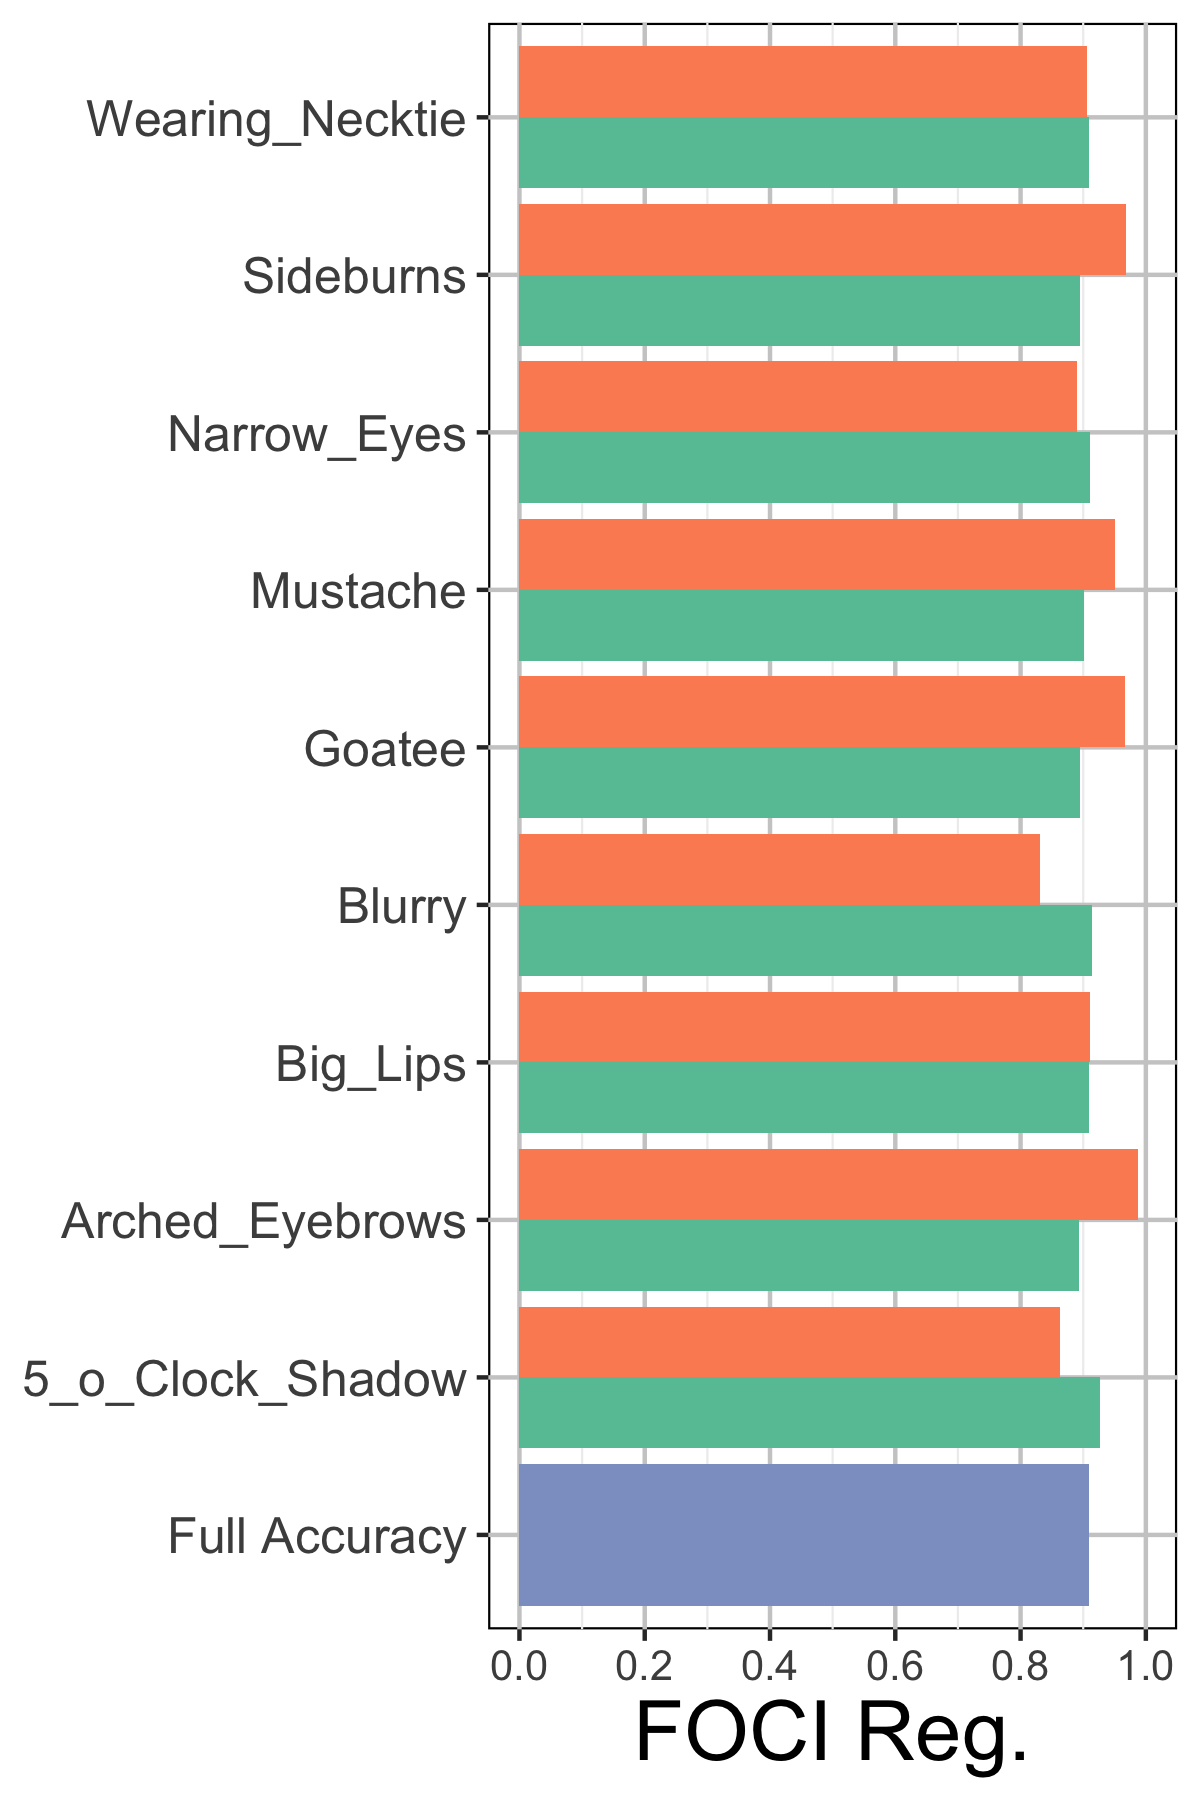
\includegraphics[width=0.3\textwidth]{figs/No_Beard_FOCI.png}
%     \caption{\label{fig:spur} Validation Accuracies on subsets of data for a model trained to predict the binary attribute ``No Beard" in the CelebA dataset. From left to right, regularization for all features, regularization for a random subset, and regularization via FOCI. Green indicates accuracy on the data with that feature, red, without.}
% \end{figure*}